% ===========================================================================
% Where to Stop: Tile-Adaptive Early Exit in a Learned Image Decoder
%
% Numbers are NOT typed into this file. Tables come from tables/*.tex and inline
% scalars from tables/macros.tex, both generated by scripts/make_paper_tables.py
% out of the measurement files in results/. Regenerate after any re-measurement.
%
% The supplement is a separate document, paper/supplementary.tex, whose sections
% are lettered A to H. Where this file points at one of them it names the
% letter, because the two documents are compiled separately and no \ref crosses
% between them.
% ===========================================================================
\documentclass[10pt,twocolumn,letterpaper]{article}

\IfFileExists{cvpr.sty}{\usepackage{cvpr}}{\usepackage{cvpr_fallback}}
\usepackage{amsmath,amssymb,amsfonts}
\usepackage{graphicx}
\usepackage{booktabs}
\usepackage{multirow}
\usepackage{xcolor}
\usepackage[pagebackref=false,breaklinks=true,colorlinks,
            linkcolor=blue!60!black,citecolor=blue!60!black,
            urlcolor=blue!60!black]{hyperref}

\newcommand{\BandUseHigh}{9}
\newcommand{\BandUseLow}{45}
\newcommand{\Ceiling}{41.9}
\newcommand{\FloorHigh}{0.072}
\newcommand{\FloorLow}{0.036}
\newcommand{\GmacAtBudget}{338}
\newcommand{\IntraGmac}{453.5}
\newcommand{\MainHighRate}{18.8}
\newcommand{\MainLowRate}{33.2}
\newcommand{\MainMean}{25.4}
\newcommand{\MapBits}{89}
\newcommand{\MapOverheadLow}{0.011}
\newcommand{\NumSeq}{40}
\newcommand{\SatHigh}{0.396}
\newcommand{\SatLow}{0.179}
\newcommand{\SatWindowHi}{0.194}
\newcommand{\SatWindowMb}{15}
\newcommand{\SeamArlsHigh}{0.197}
\newcommand{\SeamLinearHigh}{0.384}
\newcommand{\SeamReplHigh}{0.218}
\newcommand{\SeamZerosHigh}{0.677}
\newcommand{\TilingOverhead}{8.5}
\newcommand{\WallMasked}{9.9}
\newcommand{\WallPredicted}{35.3}
\newcommand{\WallSorted}{28.5}


\newcommand{\dB}{\,dB}
\newcommand{\note}[1]{\textcolor{red}{[#1]}}

\title{Where to Stop: Tile-Adaptive Early Exit in a Learned Image Decoder}
\author{Anonymous CVPR submission\\ Paper ID ****}

\begin{document}
\maketitle

% =========================================================== abstract
\begin{abstract}
Learned image decoders spend the same computation on every region of a frame,
whatever that region contains. We show that decoding compute can instead be
allocated spatially, by content, with the encoder, the entropy model and the
transmitted representation left untouched. We add a multi-exit ladder to the
intra decoder of DCVC-UF, so that tiles of one frame leave a shared
reconstruction trunk at different depths. On \NumSeq\ CTC intra frames, one from
each sequence, under a $0.1\dB$ quality constraint this removes \MainLowRate\%
to \MainHighRate\% of decoder multiply-accumulates across the rate range,
\MeanAtOne\% on average, at a BD-Rate cost of \BdRateALow\%. At $0.2\dB$ the
mean saving is \MeanAtTwo\% and at $0.3\dB$ it is \MeanAtThree\%, within $0.9$
points of the ladder's \Ceiling\% architectural ceiling.

Adaptive decoding works only inside a finite window. Tiling sets a rate-dependent
quality floor below which no allocation is feasible, and a saturation point above
which every tile already sits on the cheapest path. Rescaling the budget between
those two limits collapses five rate curves that differ by \BandRawSpread\ points
onto one within \BandSpreadMean. Finally, the bits the entropy model has already
spent on a tile predict how deep that tile must decode better than a trained
\RouterParams-parameter router does, by up to \RateRankBeatsBy\ points, with no
parameters and nothing added to the file. It wins while agreeing with the
oracle's choice on fewer tiles than the head does, which suggests that
exit-label accuracy is the wrong objective to train a router on and that the
ordering is what a router has to get right. On this decoder, the bits already
spent on a region say how much computation reconstructing it needs.
\end{abstract}

% =========================================================== introduction
\section{Introduction}

Learned codecs are compared on rate and distortion, with complexity given as a
single number, so many GMAC per frame or so many milliseconds. That number is a
constant. A learned decoder runs the same graph on a page of text as on a
cloudless sky, although the sky is much the easier picture.

Classification networks abandoned this a decade ago. Early-exit
architectures~\cite{branchynet,msdnet,sdn} attach classifiers at intermediate
depths and stop as soon as the prediction is confident, and the literature
around them is by now mature~\cite{scardapane2020,eesurvey,ztw}.
Super-resolution adopted the same idea spatially: ClassSR~\cite{classsr} routes
image patches to networks of different capacity by difficulty, and
APE~\cite{aptnet} exits patches at different depths of one network. Learned
compression has taken a different route. Slimmable
autoencoders~\cite{slimcae,slimvc} give one model several complexity levels, but
the level is chosen \emph{per stream} rather than per region, and switching it
changes the bitstream.

We ask the spatial-adaptivity question inside a learned decoder, under a
constraint that makes the answer deployable: \textbf{the encoder is frozen and
the coded payload is unchanged}. That rules out re-training the analysis
transform, changing the entropy model, or altering the latent, and leaves one
place to spend adaptivity, the synthesis transform.

\begin{figure*}[t]
\centering
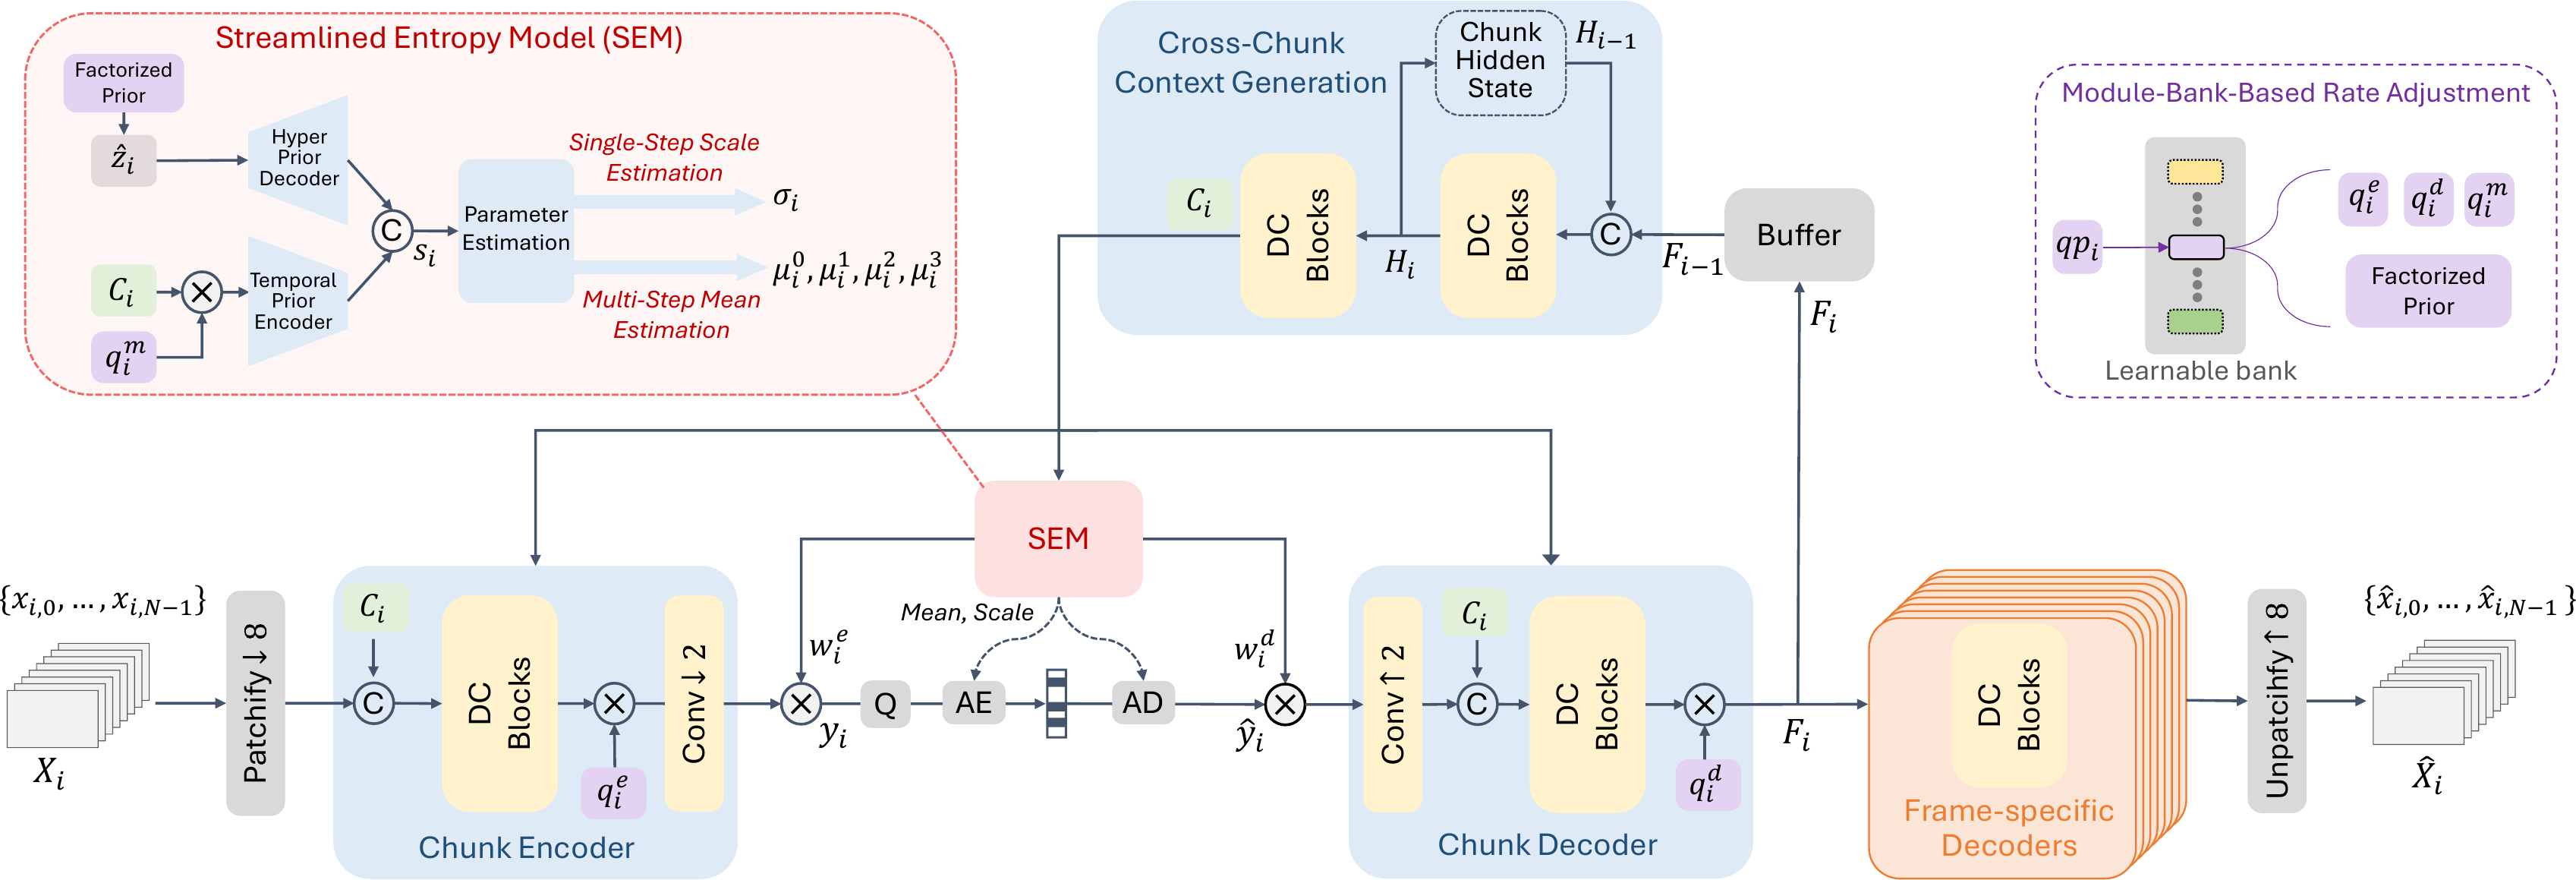
\includegraphics[width=\textwidth]{figures/dcvcuf_framework.png}
\caption{\textbf{The decoder we modify.} Figure~3 of DCVC-UF~\cite{dcvcuf},
reproduced. Everything up to the reconstruction stays frozen in this work: the
patch embedding, the chunk encoder, the entropy model and the coded payload.
FLEX-UF replaces the frame-specific decoders on the right with a ladder of exits
taken per tile.}
\label{fig:baseline}
\end{figure*}

Our method, FLEX-UF (Fig.~\ref{fig:baseline}), attaches exits at intervals
through the twelve residual blocks of the DCVC-UF intra decoder; we call that
ordered set of exits the \emph{ladder}. The first $j$ blocks run over the whole
frame. The rest run per tile, over a set of tiles that shrinks with depth, and
the shrinkage is where the saving comes from. Each exit hands its feature to the
shared head through a small pointwise adapter, zero-initialised so that at step
zero the deepest exit reproduces the released decoder bit-exactly. Getting this
to work depended less on the ladder than on two problems that have little to do
with early exit as it is usually studied.

\paragraph{Tiling has a large price.} Spatial adaptivity needs tiles, and once a
frame has been cut into tiles, every $3\times3$ convolution at a tile border
reads invented values. The tile-boundary artefact that follows is what we call
the \emph{seam}, and under the default padding rule it costs
\SeamZerosHigh$\dB$ on this decoder at high rate. That is several times the
entire budget the method works to, and it is paid before any tile has saved a
single operation. Section~\ref{sec:seam} measures what the penalty depends on,
which is not the affected area, and what removes it.

\paragraph{A distortion budget only works inside a band.} Tiling costs something
even when nothing exits early, so there is a \emph{floor}, and budgets below it
admit no allocation at all. The ladder also has a shallowest usable exit, so
there is a \emph{saturation} point above which every tile already takes that
exit and more quality buys nothing. Between the two, in what we call the
\emph{band}, the budget genuinely trades quality for compute. We measure both
ends at every rate in Section~\ref{sec:operating}, where the $0.1\dB$ budget
uses \BandUseLow\% of the band at low rate and \BandUseHigh\% at high rate.

\paragraph{The free baseline wins, and what that says about routers.} The
decoder is already holding a number that says how hard each tile was: the bits
the entropy model spent on that tile's latents, available before the trunk
starts and at no cost. A rule calibrated on that number, with no learned
parameters in it, saves more decoder arithmetic than our
\RouterParams-parameter head at every one of the \RateRankNWins\ rates we
measure, by up to \RateRankBeatsBy\ points, and it charges the decoder nothing
where the head charges \RouterCostPct\% of the decode
(Section~\ref{sec:raterank}). The part we did not expect is that it wins while
agreeing with the Lagrangian oracle's chosen exit on \emph{fewer} tiles than the
head does. Agreement over exit labels weighs a tile whose two best exits are
within a hair of each other exactly as heavily as one that carries most of the
frame's error, and most tiles are the first kind. What a router has to get right
is the order in which tiles want depth, and label accuracy is a poor stand-in
for it.

\paragraph{Contributions.}
\begin{enumerate}\itemsep2pt
\item An early-exit ladder for a learned image decoder that picks a depth per
      tile, which is spatial adaptivity at the granularity of a tile. The
      encoder, the entropy model and the coded latent are untouched in both
      modes we report. \emph{Signalled} FLEX-UF leaves the latent unchanged and
      adds \MapBits\ bits per 1080p frame of routing metadata, or
      \MapOverheadLow\% of a typical bitrate, and saves \MainLowRate\% to
      \MainHighRate\% of decoder MACs for $0.1\dB$ on the common test set at a
      BD-Rate cost of \BdRateALow\%. \emph{Bitstream-identical} FLEX-UF adds
      nothing at all, decodes a byte-identical file, and reaches
      \RouterLowRate\% to \RouterHighRate\%.
\item The band a distortion budget works in: a floor below which no allocation
      is feasible and a saturation point above which none improves, both in
      closed form. Measuring the budget in units of that band accounts for most
      of the rate dependence, on two independently trained checkpoints.
\item A zero-learned-parameter control that adaptive-inference work is rarely
      measured against, and which we report as a result rather than as a
      baseline. Routing on the bits the entropy model has already spent per tile
      costs nothing, adds nothing to the stream, and beats our trained head at
      every rate, while agreeing with the Lagrangian oracle on fewer tiles than
      the head does. The quantity that decides a router is the ranking it
      induces over tiles, and exit-label accuracy tracks it poorly.
\end{enumerate}

% =========================================================== related work
\section{Related work}

\paragraph{Early exit.} BranchyNet~\cite{branchynet} and MSDNet~\cite{msdnet}
established the pattern of intermediate classifiers with a confidence rule;
SDN~\cite{sdn} framed it as mitigating overthinking, and ZTW~\cite{ztw} recycles
earlier predictions. We train all exits jointly, after
Scardapane~\etal~\cite{scardapane2020}, and distil between \emph{adjacent} exits
as in Phuong and Lampert~\cite{phuong2019}, since too large a student--teacher
gap hurts the shallowest exits~\cite{msd2024}. All of this work exits on a
confidence signal computed from the network's own output. A decoder has no such
signal: there is no class posterior, and the quantity that would decide is the
error against a source the decoder cannot see (Section~\ref{sec:alloc}).

\paragraph{Spatially adaptive inference.} ClassSR~\cite{classsr} sorts
super-resolution patches into easy/medium/hard and runs a different network on
each; APE~\cite{aptnet} exits patches at different depths;
Glance-and-Focus~\cite{glancefocus} spends resolution adaptively. We share the
per-region premise with all three, and we inherit the same tiling problem,
though the cost of tile borders is rarely quantified in that line of work. The
closest prior work on the border itself is the per-channel AR(1) padding of
Kaseva~\etal~\cite{arls}, which we implement and evaluate.

\begin{table}[t]
\centering
\resizebox{\columnwidth}{!}{\begin{tabular}{lllccc}
\toprule
Method & Varies & Where & Latent & Side & Dec. \\
 & & & & data & only \\
\midrule
SlimCAE~\cite{slimcae} & width & per stream & new & -- & no \\
Slimmable video~\cite{slimvc} & width & per stream & new & -- & no \\
EVC~\cite{evc} & mask / pruning & per model & new & -- & no \\
Spatial competition~\cite{spatialcompetition} & which codec & per region & new & yes & no \\
DCVC-RT~\cite{dcvcrt} & architecture & fixed & new & -- & no \\
\textbf{FLEX-UF} signalled & \textbf{decoder depth} & \textbf{per region} & \textbf{same} & \MapBits\,b & no \\
\textbf{FLEX-UF} bitstream-identical & \textbf{decoder depth} & \textbf{per region} & \textbf{same} & \textbf{none} & \textbf{yes} \\
\bottomrule
\end{tabular}
}
\caption{\textbf{Where this sits.} What each method varies, at what
granularity, and what that costs the stream. A single new-bitstream column
cannot represent our own two modes, so the last three ask what actually changes:
whether the coded latent is new, what side data travels with it, and whether a
decoder alone can do it.}
\label{tab:positioning}
\end{table}

\begin{table}[t]
\centering
\resizebox{\columnwidth}{!}{\begin{tabular}{lrrr}
\toprule
Method & kMAC/px & Par. (M) & BD-Rate (\%) \\
\midrule
CHARM~\cite{charm} & 496 & 58.5 & $+0.86$ \\
STF~\cite{stf} & 511 & 99.9 & $-2.06$ \\
ELIC~\cite{elic} & 574 & 36.9 & $-3.22$ \\
WeConvene~\cite{weconvene} & 2343 & 107.2 & $-6.98$ \\
MambaVC~\cite{mambavc} & 814 & 47.9 & $-8.72$ \\
DCVC-DC intra~\cite{dcvcdc} & 542 & 45.5 & $-9.18$ \\
TCM~\cite{tcm} & 1824 & 76.6 & $-10.70$ \\
FLIC~\cite{flic} & 1096 & 71.0 & $-13.20$ \\
MLIC++~\cite{mlicpp} & 1283 & 116.7 & $-15.15$ \\
HPCM-Base~\cite{hpcm} & 919 & 68.5 & $-15.31$ \\
HPCM-Large~\cite{hpcm} & 1261 & 89.7 & $-19.19$ \\
\bottomrule
\end{tabular}
}
\caption{\textbf{What a learned image decoder costs.} Eleven codecs as
published, measured on one machine by Li et al.~\cite{hpcm}: BD-Rate against
VTM-22.0 on Kodak, arithmetic per pixel and parameters. The spread in cost is an
order of magnitude, and every entry pays its cost on every pixel of every image.}
\label{tab:litimg}
\end{table}

\begin{table}[t]
\centering
\resizebox{\columnwidth}{!}{\begin{tabular}{lrrrc}
\toprule
Method & GMAC & Par. (M) & BD-Rate (\%) & Adaptive \\
\midrule
DCVC-DC~\cite{dcvcdc} & -- & 18.3 & $+14.5$ & no \\
DCVC-FM~\cite{dcvcfm} & 2642 & 18.3 & $-21.3$ & no \\
DCVC-RT~\cite{dcvcrt} & 385 & 20.7 & $-21.0$ & no \\
DCVC-UF (LD)~\cite{dcvcuf} & 170 & 9.7 & $-9.5$ & no \\
DCVC-UF (HT-S)~\cite{dcvcuf} & 211 & 81.2 & $-31.6$ & no \\
DCVC-UF (HT-L)~\cite{dcvcuf} & 343 & 120.5 & $-42.2$ & no \\
\midrule
\textbf{FLEX-UF} intra decoder & \textbf{\RelKMacPx$\,\to\,$\OursKMacPx} & -- & \textbf{$+$\BdRateALow} & \textbf{yes} \\
\bottomrule
\end{tabular}
}
\caption{\textbf{The family this work modifies}, from DCVC-UF~\cite{dcvcuf}:
MACs per 1080p frame, parameters, and BD-Rate against VTM-17.0 low delay.
Comparable within this table and not against Table~\ref{tab:litimg}, which uses
a different anchor and a different test set. The last column is the one this
paper is about: whether the decoder spends more computation where the picture
needs it. Our row is the intra decoder of the last DCVC-UF entry, at the
$0.1\dB$ budget.}
\label{tab:litvid}
\end{table}

Table~\ref{tab:positioning} places this work against the methods above.
Tables~\ref{tab:litimg} and~\ref{tab:litvid} say where the field spends its
decoder budget.
Complexity has moved a long way in both directions: \cite{tcm} and
\cite{weconvene} buy rate with an order of magnitude more arithmetic per pixel
than \cite{charm} or \cite{stf}, and DCVC-UF~\cite{dcvcuf} moves the other way,
cutting a 1080p frame from DCVC-FM's $2642$ GMAC to $170$. Two things are
constant down both tables. The cost is a property of the model, chosen once and
paid on every image; and it is uniform over the frame, so a flat sky and a face
are decoded at the same price. Those are the two the ladder in this paper
changes, and it changes them without touching the model that was shipped.

\paragraph{Complexity control in learned compression.} SlimCAE~\cite{slimcae}
and slimmable video codecs~\cite{slimvc} expose several widths of one model, per
stream and by changing the encoder. DCVC-FM~\cite{dcvcfm} and
DCVC-UF~\cite{dcvcuf} reduce cost architecturally, for every frame equally.
Rate--distortion--complexity has since become an explicit third
axis~\cite{gao2024rdc,ho2024rdctradeoffs}, and Zhang and
Gao~\cite{zhang2025raterouting} route \emph{whole frames} to one of several
jointly-trained coding paths. Every one of these changes the model, and with it
what the encoder emits. Our axis is orthogonal: the model and the bitstream are
both fixed, and only \emph{how much of the decoder runs where} varies.

\paragraph{The closest neighbour.} Blard~\etal~\cite{spatialcompetition} also
partition an image into regions, also choose per region by a rate--distortion
cost computed at the encoder, and also transmit a mode map. Their regions choose
among several \emph{separately trained} codecs, so the decoder must hold all of
them and its complexity is that of one codec regardless of the choice; the map
buys rate, not compute. Ours choose a prefix length of a single trunk, so the
weights are shared by construction and the map buys compute at fixed rate.
Because their alternatives are unrelated networks, no decoder-side predictor
could stand in for the encoder's search. Our exits are prefixes of one another,
and that nesting is what lets a decoder-side predictor stand in at all
(Section~\ref{sec:setting}).

\paragraph{Signalling versus prediction.} Being \emph{told} a mode decision
rather than inferring it is the norm in standardised video coding.
HEVC~\cite{hevc} and VVC~\cite{vvc} transmit partitioning, prediction mode and
transform tree. We evaluate both, and treat the signalled variant as the
conventional design (Section~\ref{sec:setting}).

\paragraph{Allocating a budget over units.} The construction we use is not new
and we do not present it as such. Shoham and Gersho~\cite{shoham1988} showed
that for a finite set of per-unit operating points, a Lagrangian sweep decouples
the allocation across units and traces exactly the lower convex hull of the
achievable set; Ortega and Ramchandran~\cite{ortega1998} made it standard
practice in image and video coding. What we add is the structure this particular
operating set has: a floor below which no allocation is feasible and a
saturation point above which none improves
(Section~\ref{sec:operating}). The same relaxation has resurfaced for test-time
compute in language models~\cite{ctca}, with per-instance decoupling and a
binary search on the multiplier. That is the identical structure in a domain
with no rate axis, and it suggests that the floor and saturation
characterisation is worth stating beyond this decoder.

\paragraph{How much is there to gain?} Bounding what adaptive inference could
achieve is itself a line of work. Hasan~\etal~\cite{adaptivelimits} derive an
oracle bound on efficiency at fixed accuracy and report $43$--$121\times$ on
ImageNet. Their bound has a ceiling and no floor, because the largest model in
their family reaches the reference accuracy by definition. Spatial adaptivity
introduces a floor: cutting a frame into tiles costs quality even when every
tile runs to full depth, so the reference is unreachable at \emph{any} compute
and the feasible set of budgets is an interval rather than a ray.
Section~\ref{sec:operating} characterises that interval and both of its ends.

\paragraph{Tile boundaries.} Every method that processes an image in
independently-computed tiles meets the same artefact. The remedies in the
literature are overlap and averaging, local padding from neighbouring
patches~\cite{localpadding}, training with overlaps~\cite{overlaptrain}, and
fitted extrapolation~\cite{arls}. Local padding is the closest to the exact
remedy we measure in Section~\ref{sec:coupling}, and the difference is
accounting: it pads every convolutional layer and does not report the cost. To
our knowledge the estimator view of the padding rule and the dependence of the
penalty on per-tile depth (Section~\ref{sec:seam}) have not been reported.

\paragraph{Where the time goes.} DCVC-RT~\cite{dcvcrt} argues that operational
rather than computational complexity is the speed bottleneck for neural codecs.
Section~\ref{sec:wallclock} is an instance of that claim inside one loop:
removing \WallPredicted\% of the operations buys \WallSorted\% of the time, and
\WallSortedGain\ points of the difference come back from reordering the loop
with the arithmetic untouched.

% =========================================================== method
\section{A tile-adaptive decoder on a frozen latent}
\label{sec:method}

\subsection{Setting and notation}
\label{sec:setting}

\paragraph{The decoder.} We work on the intra decoder of DCVC-UF~\cite{dcvcuf}.
The analysis side stays frozen throughout: the patch embedding, the chunk
encoder, the entropy model and the coded payload are never touched
(Fig.~\ref{fig:baseline}). What we replace is the synthesis trunk that turns the
decoded latent into a picture. We call the unmodified public decoder the
\emph{released decoder}, and one full-frame run of it is the unit of both cost
and quality below.

\paragraph{Tiles and exits.} A frame is cut into square tiles, $256$\,px on a
side unless we say otherwise, and each tile is carried through part of the trunk
on its own. Tiles are indexed by $t$ and there are $N$ of them, $N{=}40$ at
1080p, and what they lose at a given depth is not the same from one to the next
(Fig.~\ref{fig:unequal}). The trunk itself is a stack of twelve blocks; we cut it into $K$ groups
and attach an exit to each, so exits are indexed by $k$ and exit $K-1$ is the
whole trunk. The first $j$ groups run once over the whole frame and the remaining
$K-j$ run per tile, so $j$ is the \emph{split depth}. A tile that leaves at exit
$k$ runs groups $j$ to $k$ and skips everything after it. Writing $c_k$ for what
a tile costs at exit $k$, a frame that assigns exit $k_t$ to tile $t$ costs
$\frac{1}{N}\sum_t c_{k_t}$. Tiles are cut on the trunk's feature grid, which is
coarser than the pixel grid, but we quote tile sizes in pixels.

\paragraph{Distortion and the budget.} $D_{t,k}$ is the error tile $t$ incurs if
it leaves at exit $k$. It is measured on the path we deploy at inference, a
tiled decode, against the released decoder's full-frame decode of the same
latent, so what tiling costs is inside it; we call that path the \emph{deployed
path} and the table built on it the \emph{deployed table}. Tapping the exits of
one full-frame forward pass gives a cheaper \emph{full-frame table} that is not
the same quantity, and Section~\ref{sec:exp} measures the difference. Every
result is quoted at a \emph{distortion budget}, the decibels a decoded frame is
allowed to fall below the released decoder on that same latent, and the headline
budget is $0.1\dB$. To allocate is to choose an exit for every tile so that the
frame lands on its budget as cheaply as possible. Rate is set by a quality index
running from $q0$, the lowest rate, to $q63$, the highest, and we report five of
them: $q0$, $q16$, $q32$, $q48$ and $q63$.

\begin{center}\small
\begin{tabular}{@{}l p{0.74\columnwidth}@{}}
\toprule
symbol & meaning \\
\midrule
$t$, $N$ & tile index and tiles per frame; $N{=}40$ at 1080p \\
$k$, $K$ & exit index and number of exits, $k\in\{0,\dots,K-1\}$; $K{=}6$ \\
$j$ & split depth: groups $0..j{-}1$ run full frame, $j..K{-}1$ per tile; $j{=}2$ \\
$c_k$ & cost of a tile at exit $k$, as a fraction of one released full-frame decode \\
$D_{t,k}$ & error of tile $t$ at exit $k$, tiled decode against the released full-frame decode of the same latent \\
$\lambda$ & multiplier trading $c_k$ against $D_{t,k}$, bisected to the budget \\
$\beta$ & the same trade applied to the router's logits \\
$q$ & quality index, $q0$ the lowest rate and $q63$ the highest \\
\bottomrule
\end{tabular}
\end{center}

\begin{figure}[t]
\centering
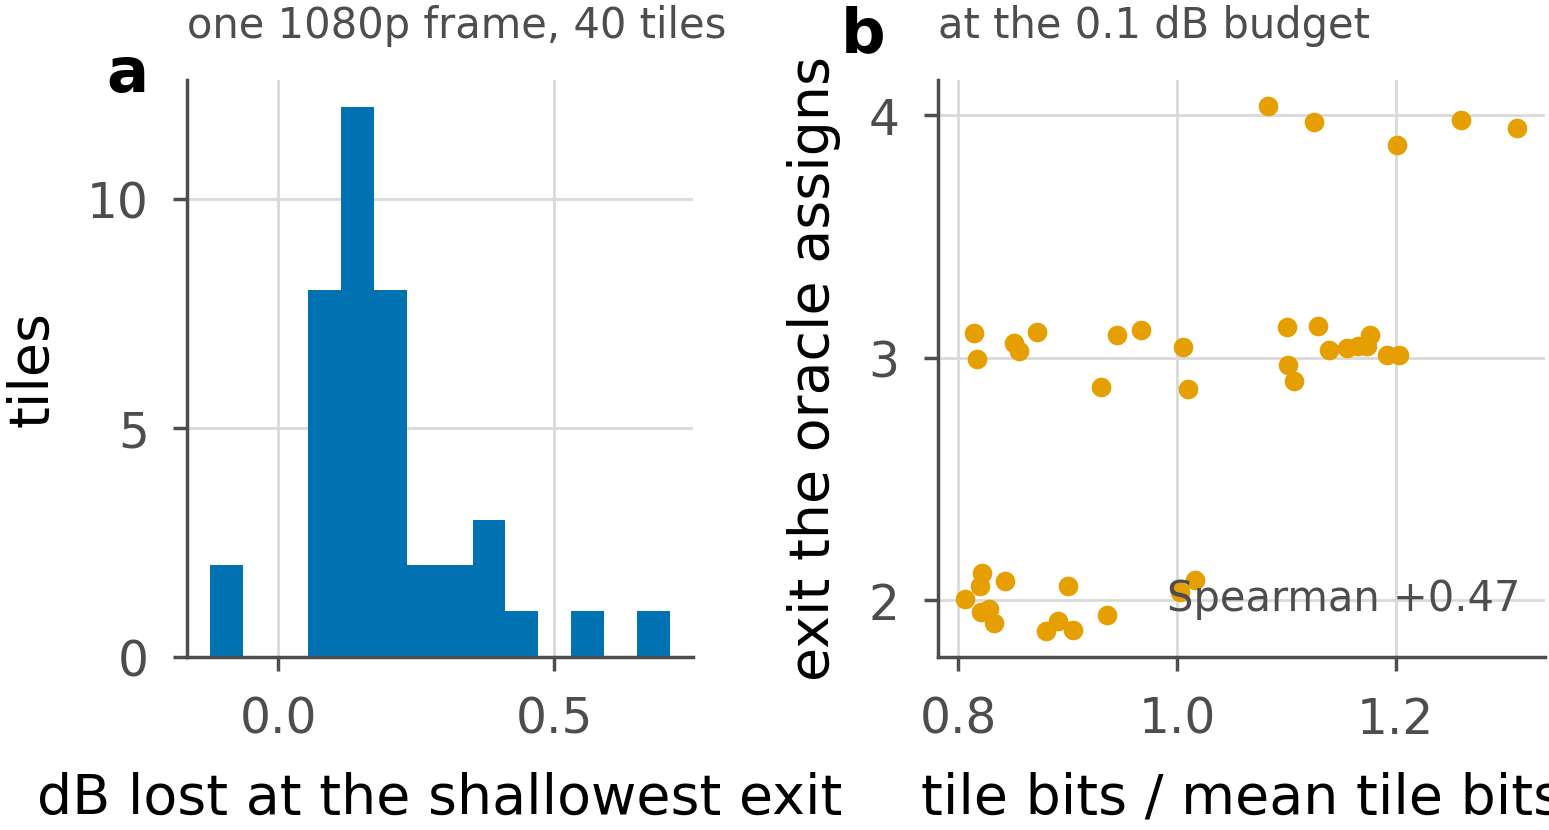
\includegraphics[width=\columnwidth]{figures/tiles_unequal.png}
\caption{\textbf{Why depth should not be uniform.} One 1080p frame, $40$ tiles.
\textbf{a}, what each tile loses if it stops at the shallowest exit the ladder
allows: several lose nothing measurable and the worst loses several times the
budget, so a single depth for the frame has to be set by the worst of them.
\textbf{b}, the bits the entropy model has already spent on a tile against the
exit the Lagrangian oracle sends it to, at the $0.1\dB$ budget. The signal a
decoder-side router needs is already in the file.}
\label{fig:unequal}
\end{figure}

\paragraph{Two deployment modes.} Both choose the same object, one exit per
tile, on the same weights and the same coded payload, and they differ only in
where that choice is made. \emph{Signalled} FLEX-UF, configuration~\textbf{A},
decides at the encoder. The encoder holds the source, so it knows $D_{t,k}$,
picks each tile's exit by the Lagrangian of Section~\ref{sec:alloc}, and
transmits the resulting \emph{exit map}, one exit index per tile, which is the
analogue of the mode map a standard codec signals. It entropy-codes to
$\sim$\MapBits\ bits per 1080p frame, or \MapOverheadLow\% of a typical bitrate;
the coded latent is unchanged. It costs the encoder about one extra decode per
frame and the decoder nothing. \emph{Bitstream-identical} FLEX-UF, configuration
\textbf{B}, decides at the decoder. A \RouterParams-parameter head reads decoded
data only and predicts the same map (Section~\ref{sec:alloc}). Nothing is
transmitted and the file stays byte for byte the one the released encoder
produced. It costs the decoder \RouterCostPct\% of its own
multiply--accumulates, which is charged inside every B number we report. Every
saving quoted in this paper is labelled with the mode it was measured in.
Because the head reads nothing the encoder cannot also read, the encoder can run
it too and so knows tile by tile where it will be wrong; supplement~G measures
the interpolation between the two modes that this allows.

\subsection{The ladder, its cost and its ceiling}

The DCVC-UF intra decoder is one upsampling block, twelve \texttt{DepthConvBlock}s
and a head, costing $\IntraGmac$ GMAC per 1080p frame. The twelve blocks are $89.4\%$
of that, which is why we build the ladder across them. Inside one block at
$C{=}384$ channels, the only operator with any spatial extent is a $3\times3$
depthwise convolution, and it costs $9C$ against the block's $8C^2 + 9C$. That is
$\mathbf{0.29\%}$, and it is the fraction the rest of this paper turns on. Tile
borders damage the picture through it, it is what makes the exact remedy of
Section~\ref{sec:coupling} affordable at all, and it is why the exit adapters are
pointwise: a $3\times3$ inside an adapter would add seam damage at exactly the
tiles that took an early exit. Supplement~A gives every adapter its shape and
measures what each is worth.

Two consequences follow from the ladder, and both are easy to state wrongly.
Exits shallower than $j$ are indistinguishable from each other, because the first
$j$ groups run for every tile regardless, and the usable ladder therefore has
$K-j$ distinct costs. The second consequence is the \emph{architectural ceiling}
\begin{equation}
S_{\max} = 100\,(1 - c_j)\;\%,
\label{eq:ceiling}
\end{equation}
reached when every tile takes exit $j$. For our shipped setting ($K{=}6$,
$j{=}2$, $256$\,px tiles) $S_{\max} = \Ceiling\%$. We show in
Section~\ref{sec:operating} that this bound is \emph{reached} in practice at low
rate, so it behaves as an operating point and not as an asymptote.

\subsection{Allocation: encoder search, decoder prediction}
\label{sec:alloc}

Every tile has to be given an exit, drawn from the usable ones, $k \ge j$, and we
want the set of choices that keeps the frame inside its distortion budget for the
least compute. There are $K-j$ choices per tile and $N$ tiles, so searching
assignments one by one is out of the question. What makes the problem tractable
is that the tiles do not interact: each contributes its own error $D_{t,k}$ and
its own cost $c_k$, and the only thing they share is the single budget the frame
has to meet. Problems of that shape are solved with a Lagrangian. Put a price
$\lambda$ on compute, add $\lambda c_k$ to the error of exit $k$, and the budget
constraint drops out; what is left is $N$ separate one-tile problems, each a
minimum over $K-j$ numbers. Compute falls and error grows as $\lambda$ grows,
neither of them turning back, so one value of $\lambda$ puts the frame exactly on
its budget and we find that value by bisection. The rule each tile follows is
\begin{equation}
k^{*}_t(\lambda) \;=\; \arg\min_k \; \bigl[\, D_{t,k} + \lambda\, c_k \,\bigr],
\label{eq:lagrangian}
\end{equation}
with the minimum taken over $k \ge j$. We call $k^{*}_t(\lambda)$ the choice of
the \emph{Lagrangian oracle}: it is made with the true error of every exit in
hand, which no decoder has, but it is optimal only within the family of
allocations one multiplier can reach. That qualifier is not cosmetic.
Supplement~G exhibits allocations that are cheaper at the same distortion than
anything this rule produces, so ``oracle'' here means best-under-a-single-%
multiplier and not the global constrained optimum. Where we mean the latter we
say so. Both quantities in~(\ref{eq:lagrangian}) are available \emph{to the
encoder}, which holds the source, so configuration~A can run this search exactly;
supplement~G prices the two ways of building the table it searches.

The decoder cannot run~(\ref{eq:lagrangian}). $D_{t,k}$ is the error against the
source, and the source is the one thing a decoder never receives. The gap is one
of information: the errors the argmin compares depend on a picture that is not in
the bitstream, so no decoder-side model recovers them, however large it is. What
a decoder can do is estimate which exit the Lagrangian oracle would have picked,
and configuration~B therefore \emph{predicts}. Its head reads what the decoder
already holds, the feature at the split point, the decoded latent $\hat{y}$, the
entropy model's scales and the quality index. For each tile $t$ it emits a vector
of logits $z_t$, one entry per exit, and the tile takes
\begin{equation}
\hat{k}_t \;=\; \arg\max_k \;\bigl[\, \log \mathrm{softmax}(z_t)_k
                                       - \beta\, c_k \,\bigr].
\label{eq:router}
\end{equation}
The first term is the head's score for exit $k$, on a log scale, which is the
currency the surprisal $-\log p$ puts it in. The second is the price on compute
that $\lambda$ carries in~(\ref{eq:lagrangian}): raising $\beta$ takes more away
from the deep exits than from the shallow ones, so more tiles are handed to cheap
exits and the frame again gets cheaper and worse. Supplement~F gives the head's
architecture, its training objective and what each of its inputs is worth.

\paragraph{Where $\beta$ comes from at deployment.} A real decoder cannot bisect
$\beta$ against the budget. It would need to know the delivered distortion, and
the distortion is measured against a source the decoder never receives, which is
the same missing variable that stopped it running~(\ref{eq:lagrangian}) in the
first place. So $\beta$ is calibrated offline, once, on a held-out set, and
shipped as a table indexed by the quality index and the budget: the decoder reads
the quality index out of the bitstream, looks $\beta$ up, and runs the argmax
in~(\ref{eq:router}) with nothing in the loop needing the source. We calibrate on
\HeldNCal\ held-out Open Images validation frames, disjoint from the training
images and from the test sequences, bisecting once per quality index and applying
the table to the test set unchanged. Section~\ref{sec:ab} reports both that
number and the one obtained by bisecting on the test set itself, and
supplement~F.5 gives the measurement of whether the table transfers, because the
difference between the two is the only honest reading of that.

% =========================================================== the seam
\section{Tiling sets a floor}
\label{sec:seam}

\subsection{The seam, and how it scales with depth}

\begin{figure}[t]
\centering
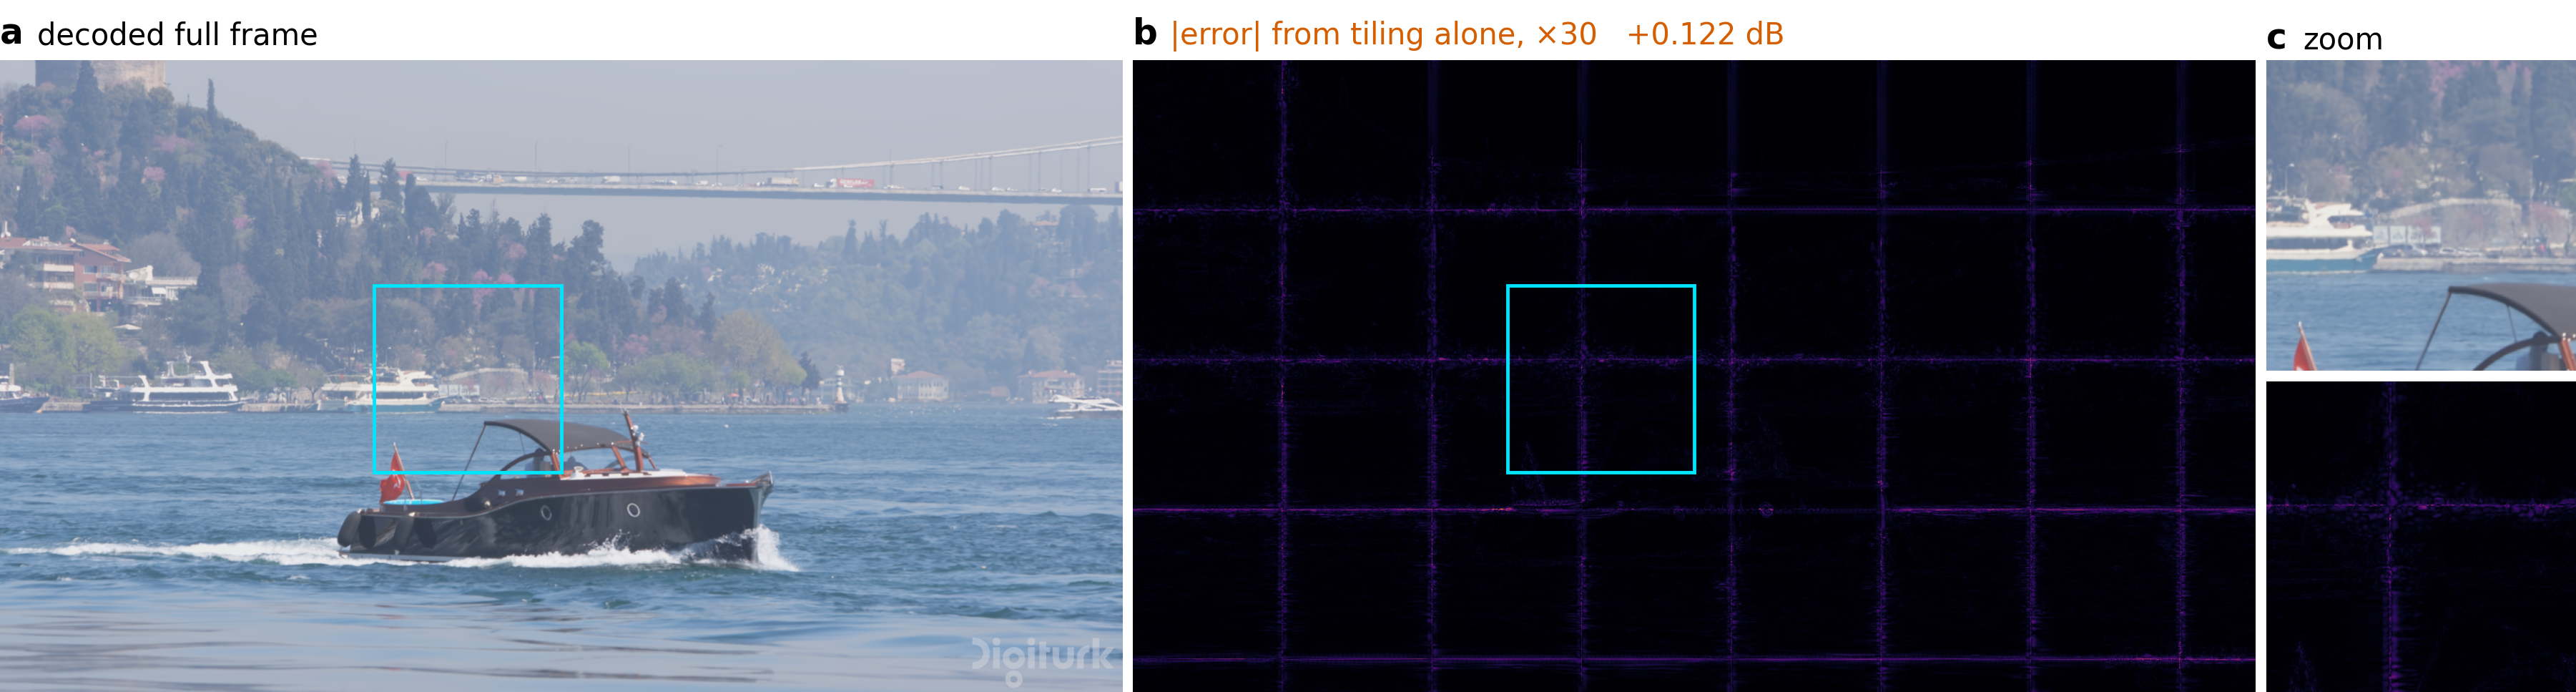
\includegraphics[width=\columnwidth]{figures/seam_problem.png}
\caption{\textbf{The artefact, before anything is done about it.} Bosphorus at 1080p,
quality index 63, zero padding at the tile border. \textbf{a}, the frame decoded
in one piece. \textbf{b}, the same bitstream and weights decoded in 256 pixel
tiles, every tile at full depth: the difference between the two, amplified 30
times. \textbf{c}, the boxed region of each.}
\label{fig:seamproblem}
\end{figure}

A $3\times3$ depthwise at feature position $(x,y)$ computes
$\sum_{u,v} w_{u,v}\, f_{x+u,\,y+v}$, over kernel offsets $u,v$ and kernel
weights $w_{u,v}$. Decoded full frame, those neighbours exist. Decoded per tile
they do not, and the kernel is handed whatever the padding rule invents. Each
convolution extends the affected region by one ring, so with $b$ per-tile blocks
on a tile of side $F$ the fraction of the tile within reach of an invented value
is $1 - ((F-2b)/F)^2$. At our shipped $F{=}32$, $b{=}8$ that comes to $0.750$.
Three quarters of the tile is affected, so what we are looking at is a structured
error over most of the tile and not a thin border at its edge
(Fig.~\ref{fig:seamproblem}).

That fraction tells us which pixels are affected and not how badly, and it turns
out to be the wrong predictor of the penalty. We swept the split depth, which
sweeps $b$ from 12 to 0 with $b{=}0$ as an exact zero-seam control, and measured
\begin{equation}
\text{seam} \;\propto\; b^{\alpha}, \qquad \alpha \approx 2,
\label{eq:contam}
\end{equation}
with $\alpha = 2.38$ at $q0$ falling to $1.93$ at $q63$. Fitted with one free
scale, the area fraction is wrong by $160$--$264\%$ where the power law is wrong
by $12$--$22\%$. The exponent has a reading. The count of affected pixels grows
like perimeter times depth, $\propto b$, and the error accumulated in each of
them grows with how many convolutions reached it, again $\propto b$. Once every
pixel has been touched the area law saturates and the penalty does not, which is
where the area law fails as a predictor.

Border padding is an \emph{estimator} of the unseen neighbour, and the seam is
its error. Supplement~A measures four of them with early exit switched off, and
the ordering is not the obvious one: a higher-order estimator is worse, because
extrapolating the local gradient past a boundary amplifies whatever noise sits on
that boundary, and the best of the four, the per-channel AR(1) fit
of~\cite{arls}, wins by about $0.02\dB$ for $10.7\%$ of decode wall-clock, which
against a $0.1\dB$ budget does not close.

\subsection{What removes it, and what does not}
\label{sec:coupling}

The largest factor of all is the easiest one to miss. On the untrained ladder,
replicate padding leaves \SeamReplHigh$\dB$ at $q63$; after training, the same
setting leaves \FloorHigh$\dB$. More than two thirds of what the estimator could
not fix is absorbed by weights learning to live with it, and that single change
removes more of the seam than any module in this paper does. Tile size is the
other free variable: a tiled decode's MAC count does not depend on it at all,
the damage scales with the tile perimeter as~(\ref{eq:contam}) predicts, and
what tile size costs is routing granularity. Supplement~A measures both, and
supplement~H reports what happened when we made the tile size track the frame
resolution.

Two modules that ought to have removed the rest did not. The first is a learned
deblocking filter, gated by position within a tile and applied once to the
stitched frame for $0.95\%$ of the decode; splitting the per-pixel error by
distance from the nearest tile boundary shows it winning on the ring nearest a
boundary and losing everywhere else, and even a perfect gate could not earn its
cost. That measurement rejects the filter's premise rather than the filter, which
is in the weights every number here was measured on and is why our deepest exit
costs $1.0095$ of a released decode; its cost is charged against every saving we
report rather than netted out. The second is the exact fix. Give the $3\times3$
its real neighbours across the tile border, a \emph{halo exchange} narrowed to
the one operator that needs it, and a tiled decode at uniform depth becomes
bit-identical to a full-frame one for $+0.032\%$ of the decode. Switched on at
inference it removes \CoupFloorDropLo--\CoupFloorDropHi\% of the floor, and it
destroys the routed allocation: at the same $0.1\dB$ budget the saving falls from
\CoupPaddedHigh\% to \CoupCoupledHigh\% at $q63$. The exchange is exact only when
every tile is at the \emph{same} depth, and routing is the deliberate violation
of that condition, so a shallow tile ends up reading a deep neighbour's
activation, an arrangement the weights have never seen. Supplement~H carries both
measurements in full.

% =========================================================== experiments
\section{The band, and what a budget buys}
\label{sec:exp}

\subsection{Protocol}

We fine-tune the decoder on $512{\times}512$ crops from
OpenImages~\cite{openimages} with the encoder frozen ($\max|\Delta| = 0$ is
asserted every run). One $\lambda_{\mathrm{rd}}$ is drawn per sample from a
log-spaced range covering all 64 quality indices, so a single set of weights
covers the whole rate range. We evaluate on \NumSeq\ intra frames, one from each
sequence of the common test set (CTC: UVG~\cite{uvg}, MCL-JCV~\cite{mcljcv} and
HEVC classes B, C, D and E).

One detail of the protocol moves the numbers enough to state on its own. The
per-tile table $D_{t,k}$ has to be built on the \emph{deployed} decode path, one
tiled decode per exit, rather than by tapping the exits of a single full-frame
forward pass. Tapping is the natural implementation and it is correct for
training, but with a full-frame reference on the other side of the ratio the
tiling penalty cancels and the quality reported is that of a decoder nobody
ships. On our model the gap is $+0.035\dB$ at the deepest exit and $+0.008\dB$ at
the shallowest, and it grows with how many blocks ran per tile, so we cannot
correct for it after the fact. The remaining conventions are fixed below; each of
them is a choice this project has at some point made both ways in different
files, and the two decibel conventions differ by a substantial fraction of the
working budget. Every number in this paper is in the convention stated, and the
alternatives are measured in supplement~E as a sensitivity study.

\begin{center}\small
\begin{tabular}{@{}p{0.26\columnwidth} p{0.68\columnwidth}@{}}
\toprule
what is fixed & what every number in this paper uses \\
\midrule
reference & the released decoder's full-frame decode of the same latent; our
side is the deployed tiled decode, so the tiling penalty sits inside every dB \\
distortion pooling & one mean squared error per frame, converted to dB, then
averaged over the \NumSeq\ frames; this is what the released codec's own
evaluation reports \\
scope of $\lambda$ and $\beta$ & one value per quality index and budget, never
per frame and never per sequence \\
the budget & applied globally: the multiplier is bisected once so that the whole
test set lands on the budget, which is what a deployment would do \\
where $\beta$ comes from & offline, on the held-out calibration frames, for a
deployable decoder; bisected on the test frames for the A-against-B comparison
in Table~\ref{tab:ab}, which supplement~F.5 then corrects \\
the mixed map & re-decoded once, and the distortion that decode delivers is what
we report; the per-exit table is used inside the search only \\
saving & counted with hooks on the executed pass, as a fraction of one released
full-frame decode \\
\bottomrule
\end{tabular}
\end{center}

The last row is worth one more sentence, because the denominator is the easiest
of these to take for granted. Our own deepest exit costs $1.0095$ of a released
decode, and dividing by that instead would flatter every result in the paper by
$0.6$--$0.8$ points.

\subsection{What a $0.1\dB$ budget buys}

\begin{table}[t]
\centering
\begin{tabular}{lrrrrrr}
\toprule
Budget & $q0$ & $q16$ & $q32$ & $q48$ & $q63$ & mean \\
\midrule
0.10\,dB & 29.2 & 25.0 & 20.4 & 17.9 & 15.2 & \textbf{21.5} \\
0.20\,dB & 38.3 & 37.0 & 33.0 & 31.0 & 28.9 & \textbf{33.7} \\
0.30\,dB & 38.3 & 38.3 & 38.3 & 37.1 & 35.0 & \textbf{37.4} \\
0.50\,dB & 38.3 & 38.3 & 38.3 & 38.3 & 38.3 & \textbf{38.3} \\
\bottomrule
\end{tabular}

\caption{\textbf{Decoder MACs saved} (\%) against the released decoder, per
quality index and distortion budget, signalled FLEX-UF. The $0.3$ and $0.5\dB$
rows sit on the architectural ceiling of Eq.~(\ref{eq:ceiling}) almost
everywhere; past that point a looser budget buys nothing.}
\label{tab:main}
\end{table}

One word on the budget before the numbers. A tenth of a decibel is an
engineering convention, chosen because it is small against the spacing of the
rate points and because codec work has long used differences of this size as a
working tolerance. It is not evidence that the difference is invisible, and we
make no perceptual claim for it. The $0.2$, $0.3$ and $0.5\dB$ rows of
Table~\ref{tab:main} are there so a reader who disagrees with the choice can
read off another one.

Table~\ref{tab:main} carries the headline numbers. At $0.1\dB$ the method saves
\MainLowRate\% at the lowest rate and \MainHighRate\% at the highest, and
\MainMean\% on average. We do not read the fall with rate as an artefact of the
ladder. High-rate reconstructions carry detail the shallow exits cannot
reproduce, and the floor rises with rate as well (Table~\ref{tab:operating});
both effects push the same way. The distribution behind those means is wide, and
supplement~D reports it per sequence: at $q0$ the median sequence saves well
above the mean while the worst saves nothing at all, and the worst cases are the
two-tile sequences, where there is almost no allocation left to make. Saving
tracks tile count more closely than it tracks content, which supplement~D
measures class by class.

\subsection{Adaptivity against its controls}

\begin{figure}[t]
\centering
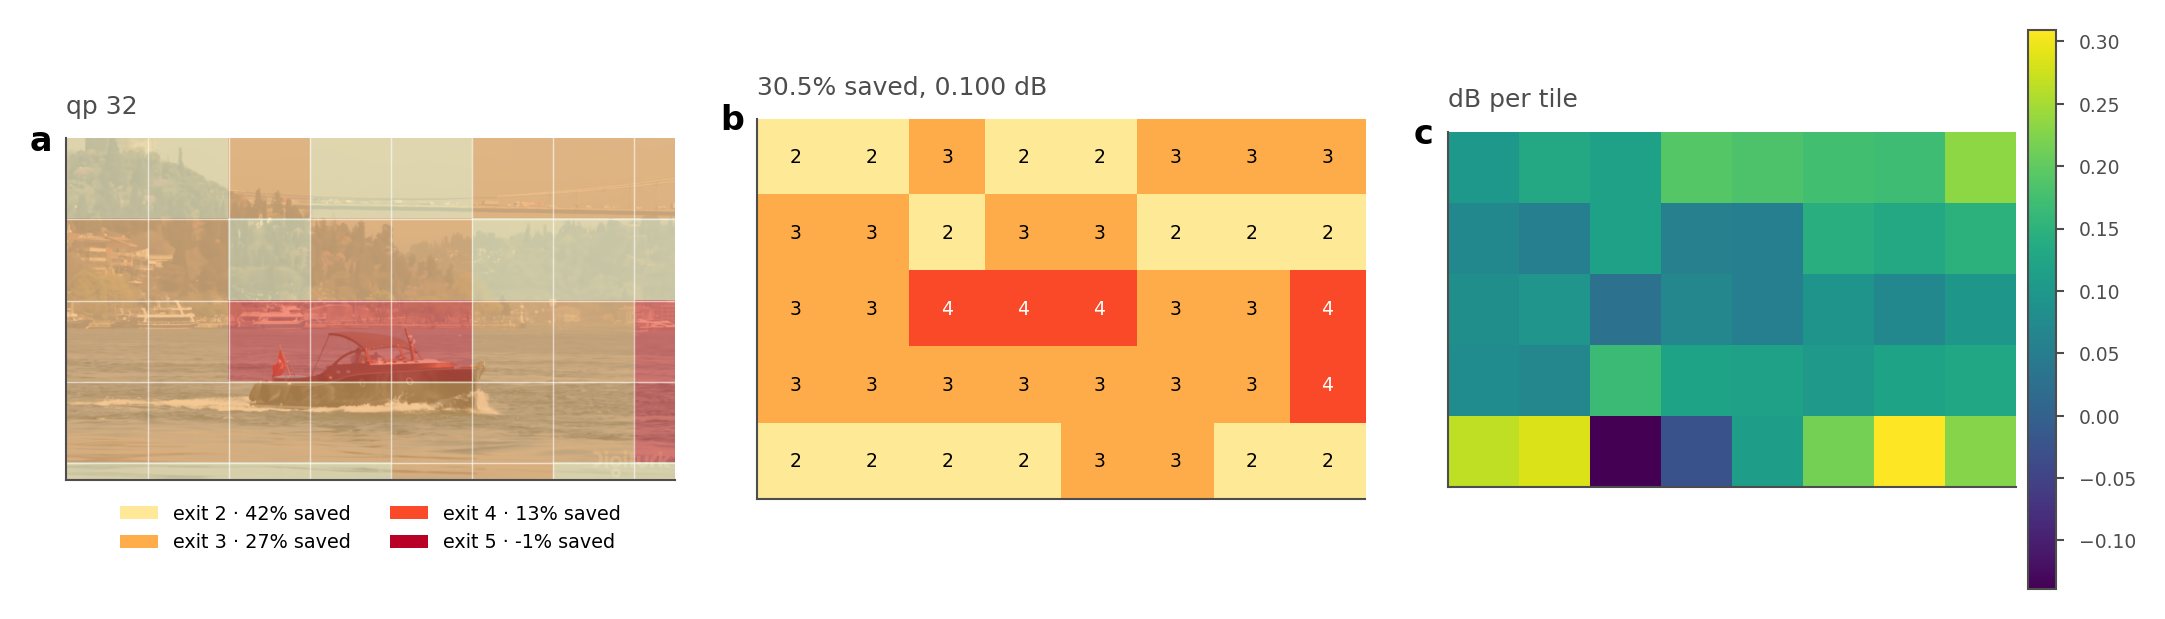
\includegraphics[width=\columnwidth]{figures/exit_map.png}
\caption{\textbf{Where the decoder spends.} Bosphorus at $q32$, a
$0.1\dB$ budget. (a) the assignment overlaid on the frame, (b) the exit index
per tile, (c) the quality each tile gives up, against its \emph{own} full-depth
reference. Water and sky leave at the shallowest exit; the boat and the
shoreline run deep.}
\label{fig:exitmap}
\end{figure}

\begin{table}[t]
\centering
\resizebox{\columnwidth}{!}{\begin{tabular}{lrrrrr}
\toprule
 & $q0$ & $q16$ & $q32$ & $q48$ & $q63$ \\
\midrule
uniform 2 & 0.139/39.1$^{\dagger}$ & 0.172/39.1$^{\dagger}$ & 0.218/39.1$^{\dagger}$ & 0.253/39.1$^{\dagger}$ & 0.288/39.1$^{\dagger}$ \\
uniform 3 & 0.061/24.2 & 0.080/24.2 & 0.105/24.2$^{\dagger}$ & 0.122/24.2$^{\dagger}$ & 0.138/24.2$^{\dagger}$ \\
uniform 4 & 0.041/13.0 & 0.055/13.0 & 0.067/13.0 & 0.074/13.0 & 0.081/13.0 \\
uniform 5 & 0.026/-1.0 & 0.034/-1.0 & 0.042/-1.0 & 0.048/-1.0 & 0.054/-1.0 \\
random & 0.114/34.5 & 0.123/30.8 & 0.134/26.7 & 0.142/25.3 & 0.147/24.1 \\
bit ranking & 0.104/34.5 & 0.104/30.8 & 0.105/26.7 & 0.107/25.3 & 0.111/24.1 \\
\textbf{oracle} & \textbf{0.100/34.5} & \textbf{0.100/30.8} & \textbf{0.100/26.7} & \textbf{0.100/25.3} & \textbf{0.100/24.1} \\
\bottomrule
\end{tabular}
}
\caption{\textbf{Adaptivity against three controls} at the $0.1\dB$ budget. Each
cell is the delivered dB over the MACs saved (\%). $^{\dagger}$ marks a uniform
depth whose distortion exceeds the budget, so it is not an admissible allocation
at all. ``Random'' draws each frame's map from the oracle's own exit histogram
and shuffles it across tiles; ``bit ranking'' keeps that histogram and orders it
by the bits the entropy model spent per tile. Both are matched to the oracle on
compute rather than on quality, which is why they carry no dagger.}
\label{tab:staticmain}
\end{table}

The obvious alternative to routing tiles is to run every tile at the same
shallower exit and accept the loss. Table~\ref{tab:staticmain} puts that option,
together with two stronger controls, at matched compute.

The uniform rows answer the question directly, and the answer sharpens with rate.
At the lowest rate a static decoder can reach exit 3 inside the budget and save
\UniformThreeLow\%, against the Lagrangian oracle's \MainLowRate\%. At $q48$ and
$q63$ the only uniform depth that fits is the deepest one, which \emph{costs}
\DeepestUniformCost\% instead of saving anything, so at those two rates the
comparison is against nothing at all rather than against something smaller.
Averaged over rates, the best static allocation saves \BestStaticMean\% where the
adaptive one saves \MainMean\%.

The two shuffled rows separate effects that are easy to conflate. Keeping the
oracle's own exit histogram leaves the mix of depths and hence the average cost
unchanged; assigning it to tiles at random makes quality fall sharply. What the
allocation buys is knowing \emph{which} tiles can afford to run shallower, and
running some fraction of them shallower is worth nothing by itself. The
oracle-histogram bit ranking keeps the same histogram and orders it by a signal
the decoder already holds, the bits the entropy model spent on each tile, which
is the cheapest router we can think of and the natural analogue of the confidence
rules early-exit classifiers use~\cite{branchynet,msdnet}. It recovers most of
the gap: at $q63$, random costs \RandomDb$\dB$ and the Lagrangian oracle
\OracleDb$\dB$ at identical compute, while the bit ranking costs
\RateRankDb$\dB$,
which is \RateRankRecovers\% of the oracle's advantage over chance. A learned
router therefore has to beat a free signal that is already three quarters of the
way there, and we would report that control in adaptive-inference work of this
kind. Given the oracle's histogram, what this measures is \emph{ranking} and
nothing else; Section~\ref{sec:raterank} removes the crutch and turns the same
signal into a complete routing rule. Fig.~\ref{fig:exitmap} shows the assignment
the oracle arrives at.

\subsection{Floor, saturation, and the band}
\label{sec:operating}

\begin{table}[t]
\centering
\resizebox{\columnwidth}{!}{\begin{tabular}{lrrrrrrrrr}
\toprule
$q$ & 0 & 8 & 16 & 24 & 32 & 40 & 48 & 56 & 63 \\
\midrule
Floor $D_{\min}$ & 0.036 & 0.040 & 0.045 & 0.050 & 0.054 & 0.059 & 0.062 & 0.066 & 0.072 \\
Saturation $D_{\mathrm{sat}}$ & 0.179 & 0.194 & 0.219 & 0.251 & 0.282 & 0.305 & 0.333 & 0.365 & 0.396 \\
Usable band & 0.143 & 0.154 & 0.174 & 0.201 & 0.228 & 0.246 & 0.271 & 0.299 & 0.324 \\
0.1\,dB uses & 45\% & 39\% & 31\% & 25\% & 20\% & 17\% & 14\% & 11\% & 9\% \\
\bottomrule
\end{tabular}
}
\caption{\textbf{Floor and saturation}, dB below the released decoder. The floor
is what tiling costs with no early exit at all; saturation is where every tile
reaches exit $j$ and the ceiling of Eq.~(\ref{eq:ceiling}) is reached.}
\label{tab:operating}
\end{table}

One assumption is worth naming before any of this. The argument treats the
frame's distortion as a sum over tiles, while the deblocking pass runs on the
stitched frame and therefore sees the whole exit map at once, so the tiles are
not strictly independent. We measured the size of that coupling over $60$
allocations and the largest mismatch between the separable prediction and a real
decode is $5.5\times10^{-5}\dB$, four orders of magnitude below the budget. We
proceed as if the objective were separable and treat that as measured rather than
assumed. Supplement~C states the structure of the allocation as propositions,
each checked numerically rather than asserted, and prices what the convex-hull
restriction costs against the exact Pareto set.

Two numbers bound what any budget can do (Table~\ref{tab:operating}). The
\textbf{floor} $D_{\min}$ is the distortion of a tiled decode with every tile at
full depth, which is pure tiling penalty: \FloorLow$\dB$ at $q0$, rising to
\FloorHigh$\dB$ at $q63$. A budget below it admits no allocation. The
\textbf{saturation} point $D_{\mathrm{sat}}$ is the distortion when every tile
takes exit $j$; any budget at or above it reaches $S_{\max}$, and a larger one
reaches nothing more. At $q0$ the ceiling is reached at \SatLow$\dB$, so the
architectural bound behaves as an operating point rather than as an asymptote,
and past it the limiting factor is the \emph{ladder} and not the budget. That is
an argument for a finer ladder before a looser budget, and supplement~E measures
the crossover: a ladder with twice as many exits loses at $0.1\dB$, because
splitting later puts twice as many blocks in the per-tile section
and~(\ref{eq:contam}) raises the floor, and wins by several points at $0.5\dB$,
where the shipped ladder has been pinned at its ceiling since $0.3\dB$.

\begin{figure}[t]
\centering
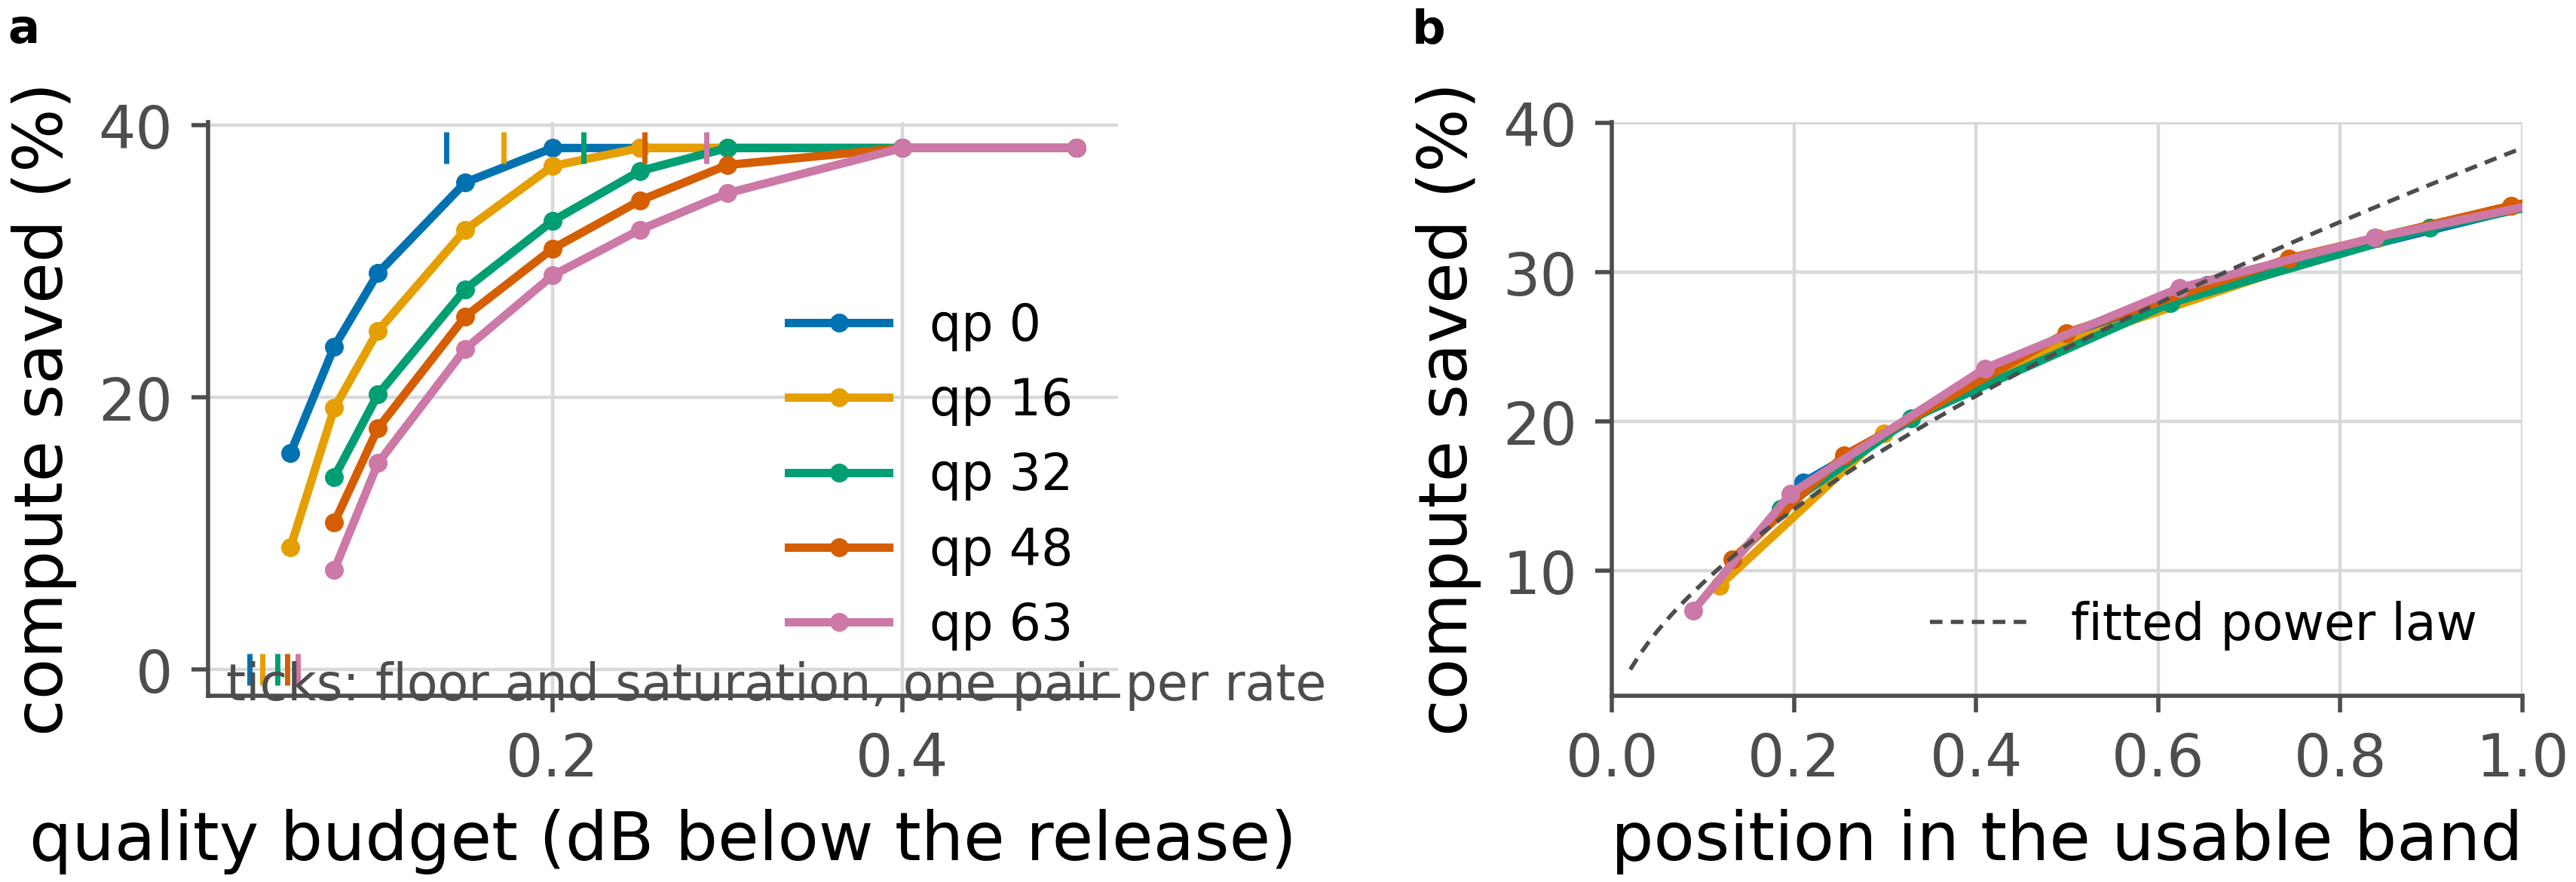
\includegraphics[width=\columnwidth]{figures/budget_band.png}
\caption{\textbf{The band is the rate dependence.} \textbf{a} Saving against the
budget, with each rate's floor and saturation point ticked. \textbf{b} The same
with the budget axis rescaled onto each rate's own band. Five curves become one; dashed is the one-parameter power law
fitted to all of them.}
\label{fig:band}
\end{figure}

The band accounts for almost all of the rate dependence. At a matched decibel the
five rates are \BandRawSpread\ points apart. Rescale the budget axis onto each
rate's own band, with the floor at $0$ and saturation at $1$, and they collapse
onto a single master curve, \BandSpreadMean\ points apart on average and
\BandSpreadMax\ at worst (Fig.~\ref{fig:band}). The answer to how much a
$0.1\dB$ budget buys at a given rate is therefore, to within a couple of points,
where $0.1\dB$ sits in that rate's band. The floor and the saturation point are
both in closed form and both cheap to measure, and what they leave over is small
enough that a deployment could calibrate the two ends and read the rest off one
curve. That curve is a one-parameter power law,
$\text{saving} \approx C\,u^{\BandExp}$, with $C$ the architectural ceiling and
$u$ the position in the band, fitted in log space over all five rates at
$R^2 = \BandRTwo$. The claim we make is the \emph{rescaling}: measuring the budget
in units of each rate's own band is what collapses the curves. The exponent is an
empirical fit to that collapse and not a law, and inverse fits to the same
frontier disagree in it by up to $40\%$, so we read nothing into its value.

The collapse appears robust across two checkpoints. We repeated the measurement
on \texttt{BEST}, a separate recipe taken at a different epoch, and the same
thing happens, with the rates \BandRawSpreadB\ points apart at a matched decibel
and \BandSpreadMeanB\ after rescaling. The \emph{exponent} does not carry over,
\BandExpB\ there against \BandExp\ here, so it describes a trained decoder and
not the architecture. What replicates is the collapse: within a checkpoint, the
rate dependence of the trade-off is the rate dependence of the band.

% =========================================================== routing
\section{Routing on bits, and real time}

\subsection{Signalled against predicted}
\label{sec:ab}

\begin{figure}[t]
\centering
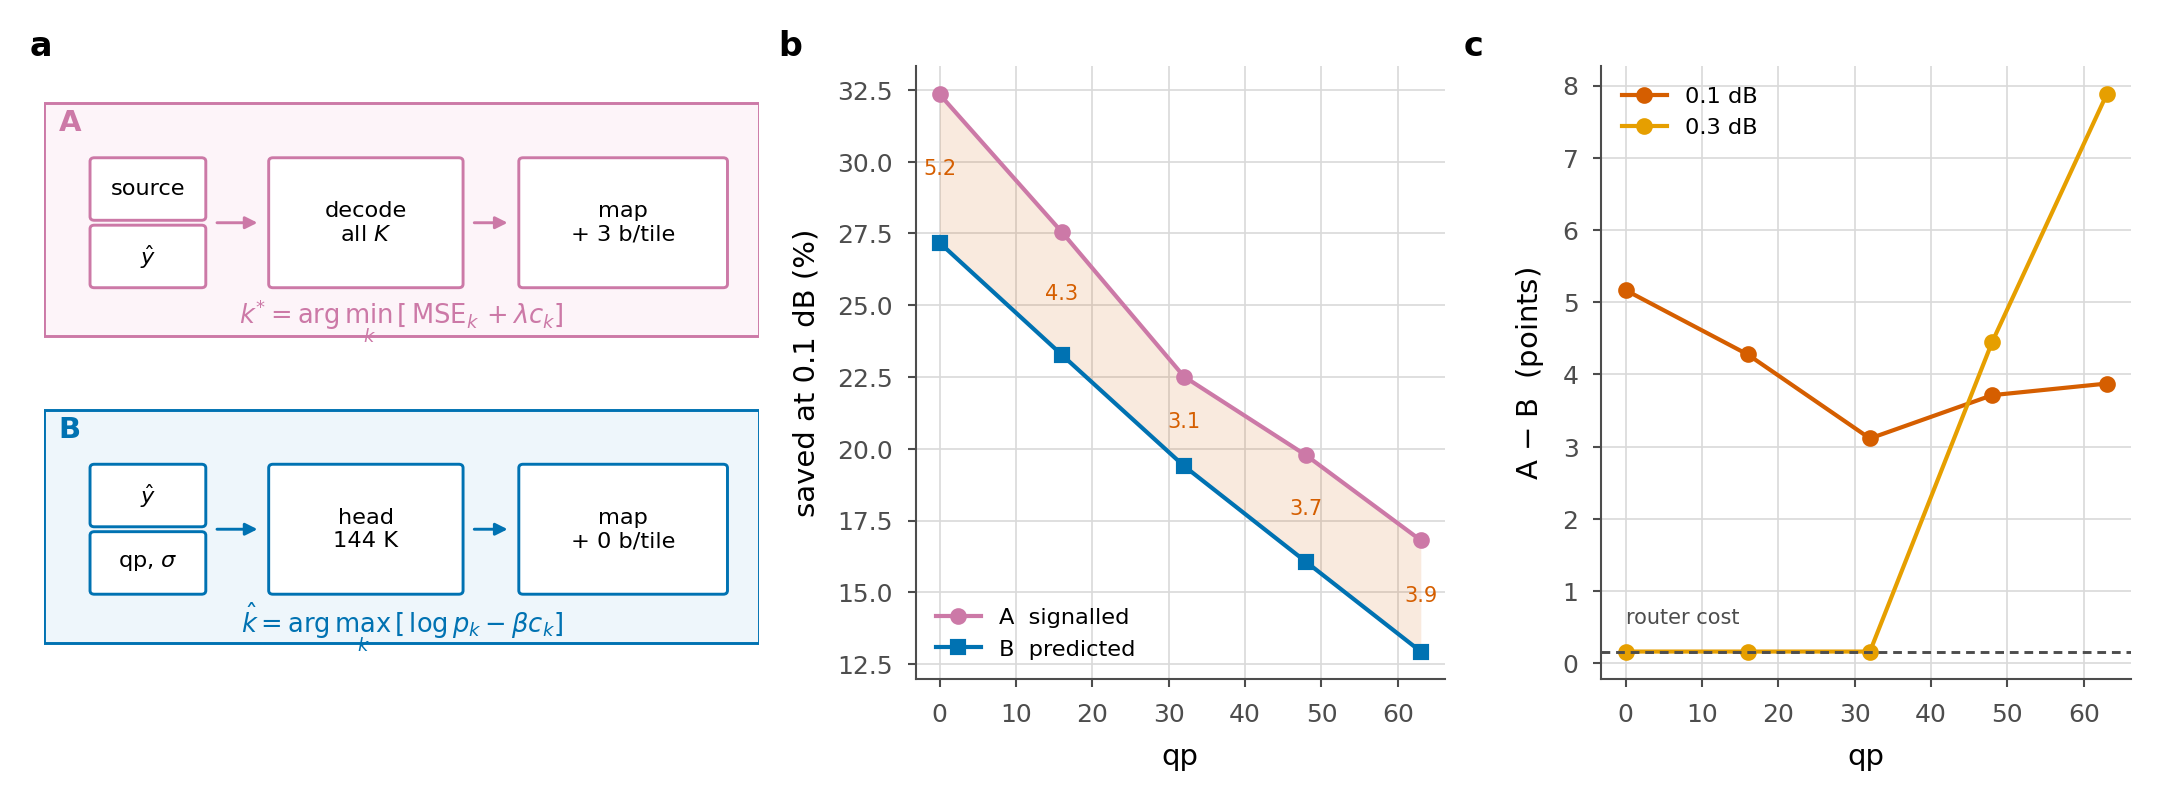
\includegraphics[width=\columnwidth]{figures/router_ab.png}
\caption{\textbf{Who decides.} \textbf{(a)} The two decision paths of
Section~\ref{sec:setting}, drawn side by side: the encoder's search over all $K$
exits per tile against the head's forward pass over decoded data.
\textbf{(b)} Saving at 0.1\,dB; shading is what a bit-exact bitstream costs.
\textbf{(c)} That cost is smallest at $q\GapMinQp$, where the router needs
almost no cost multiplier to reach the budget from where it was trained, and
grows in both directions. At $0.3\dB$ it falls to the router's own
\RouterCostPct\,\% wherever the budget saturates the ladder, and widens where it
does not.}
\label{fig:ab}
\end{figure}

\begin{table}[t]
\centering
\resizebox{\columnwidth}{!}{\begin{tabular}{lrrrrrr}
\toprule
& \multicolumn{3}{c}{0.1\,dB} & \multicolumn{3}{c}{0.3\,dB} \\
$q$ & A & B & gap & A & B & gap \\
\midrule
0 & 29.2 & 24.4 & \textbf{4.8} & 38.3 & 39.0 & \textbf{-0.6} \\
16 & 25.0 & 20.9 & \textbf{4.1} & 38.3 & 39.0 & \textbf{-0.6} \\
32 & 20.4 & 17.4 & \textbf{3.0} & 38.3 & 39.0 & \textbf{-0.6} \\
48 & 17.9 & 14.1 & \textbf{3.7} & 37.1 & 33.4 & \textbf{3.7} \\
63 & 15.2 & 11.1 & \textbf{4.1} & 35.0 & 27.7 & \textbf{7.3} \\
\bottomrule
\end{tabular}
}
\caption{\textbf{Signalled against predicted} at two budgets, same checkpoint and
test set, with one router trained against the oracle on the deployed table at a
single $\lambda$.}
\label{tab:ab}
\end{table}

Table~\ref{tab:ab} and Fig.~\ref{fig:ab} price exactness against bits. Not
signalling costs
\GapMin--\GapMax\ points, roughly flat across rate, for zero added bits and a
byte-identical file. The gap is smallest at $q\GapMinQp$ and widens toward both
ends of the rate range, tracking $|\beta|$, the cost multiplier the bisection has
to apply to move a router trained at one $\lambda$ onto another operating point.
A large $\beta$ in either direction lets the cost term dominate the logits, which
discards the content ranking the router learned. What we ship against that is one
head for every quality index, with the offline $\beta$ table of
Section~\ref{sec:alloc} in front of it: the head's ordering is what a deployment
stores, and the multiplier that moves it onto an operating point is a looked-up
scalar rather than a second set of weights. We do not propose a head per rate
anywhere in this paper, since that would multiply the stored parameters by the
number of operating points a deployment offers.

Loosening the budget closes the gap only where the budget saturates the ladder.
At $0.3\dB$ the gap is \GapLooseLow\ points at the three lowest rates, which is
exactly the router's own \RouterCostPct\% of decode, so its \emph{prediction} is
free there: both configurations send every tile to the cheapest exit and nothing
is left to predict wrongly. At the two highest rates $0.3\dB$ does not saturate
and the gap \emph{widens} to \GapLooseHigh\ points. A looser budget gives the
allocation more room to be wrong in as well as more room to be right. Every
$\beta$ in Table~\ref{tab:ab} was bisected on the test frames, which is the one
thing Section~\ref{sec:alloc} says a decoder cannot do; supplement~F.5 repeats
the measurement with the table a deployment would ship and reports where it
overshoots.

\subsection{The calibrated bit rule}
\label{sec:raterank}

\begin{figure}[t]
\centering
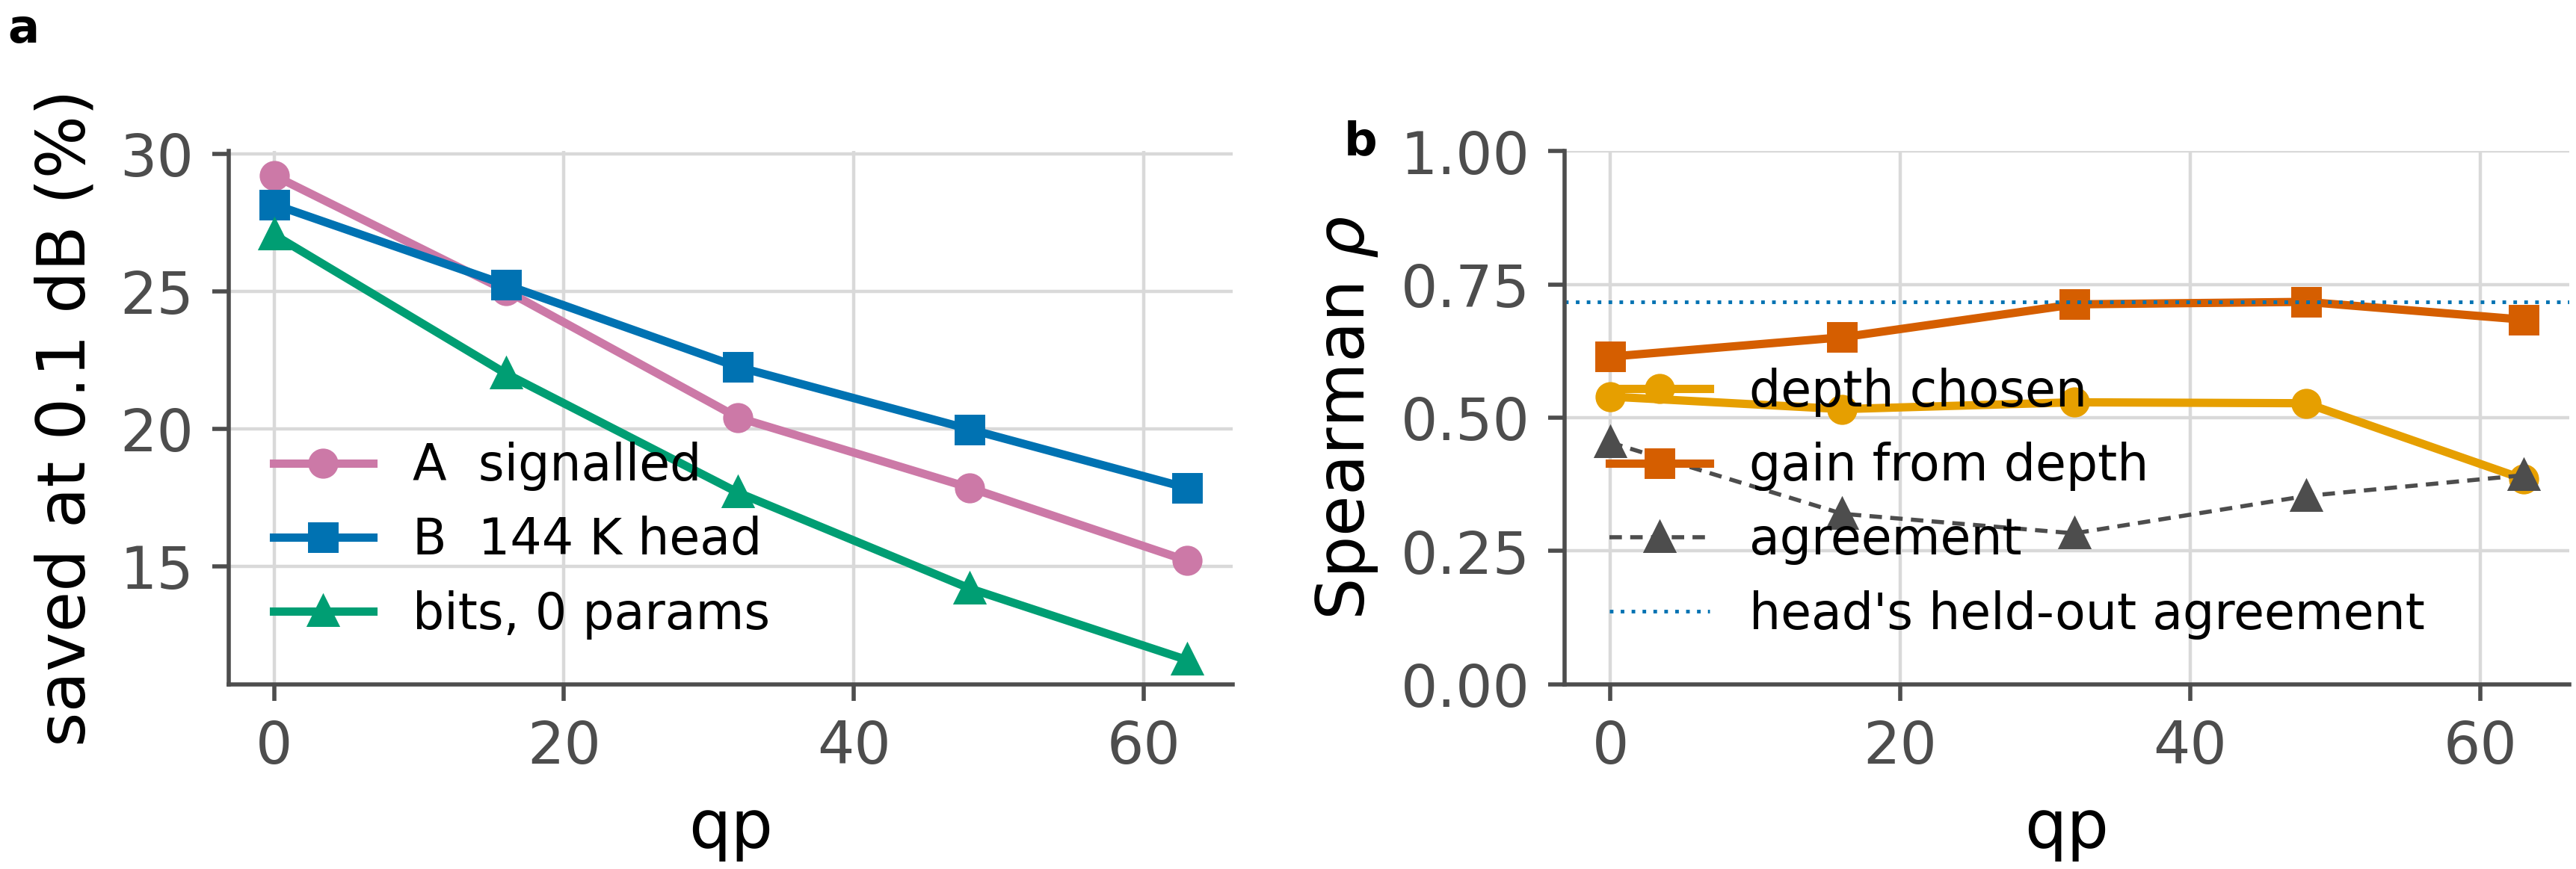
\includegraphics[width=\columnwidth]{figures/raterank.png}
\caption{\textbf{The calibrated bit rule.} \textbf{a} Saving at $0.1\dB$; shaded where
the calibrated bit rule beats the trained head. \textbf{b} What a tile's bit
count is correlated with, against how often the rule agrees with the oracle
outright; dotted is the head's own held-out agreement.}
\label{fig:raterank}
\end{figure}

\begin{table}[t]
\centering
\resizebox{\columnwidth}{!}{\begin{tabular}{lrrrrr}
\toprule
$q$ & rate-rank & B router & A signalled & $\rho$ depth & $\rho$ spread \\
\midrule
0 & \textbf{33.6} & 28.2 & 33.7 & +0.42 & +0.61 \\
16 & \textbf{29.2} & 25.2 & 30.1 & +0.46 & +0.68 \\
32 & \textbf{24.2} & 22.2 & 26.1 & +0.47 & +0.73 \\
48 & \textbf{21.4} & 20.0 & 24.8 & +0.51 & +0.80 \\
63 & \textbf{19.6} & 17.8 & 23.5 & +0.45 & +0.71 \\
\bottomrule
\end{tabular}
}
\caption{\textbf{The calibrated bit rule}, $0.1\dB$, same test set; it is the
``rate-rank'' column. Bold where the rule beats the trained head. $\rho$ are
Spearman correlations
between a tile's bit count and, respectively, the depth the oracle assigns it and
the distortion it stands to gain from that depth.}
\label{tab:raterank}
\end{table}

Before a $\RouterParams$ head is worth its \RouterCostPct\% of the decode, it has
to beat what the decoder already knows. The entropy model has produced one number
per tile before the trunk runs, and at no cost: how many bits that tile's latents
took. We turn it into a routing rule with no learned parameters by modelling the
per-tile distortion as rank-1 in the log domain,
$\log D(t,k)\approx\alpha\log b(t)+c+\log\varphi_k$, where $b$ is the tile's bit
count normalised by the frame mean and $\varphi$ is a $K$-vector saying what each
exit costs on an average tile. We fit $(\alpha,c,\varphi)$ by least squares,
leave-one-sequence-out, so that no sequence contributes to the profile that routes
it, and then run the same Lagrangian the oracle runs on the surrogate. Nothing is
signalled and nothing is trained; the arithmetic is one scalar per tile.

It beats the trained head at every rate (Table~\ref{tab:raterank},
Fig.~\ref{fig:raterank}). The calibrated bit rule is ahead of the
\RouterParams\ router at all \RateRankNWins\ measured rates, by margins that run
from half a point at $q48$ to \RateRankBeatsBy\ points at $q0$. A head trained on
this decoder against this oracle therefore returns nothing over a rule with no
parameters at all, and it carries \RouterCostPct\% of the decode that the rule
does not. It replicates on \texttt{BEST}: there the rule beats that run's own
head at \BestRankWinsN\ of \BestRankOfN\ rates, by up to \BestRankBy\ points, and
comes within \BestRankToOracle\ points of the \emph{oracle} everywhere. We do not
read that as showing a learned head cannot be worth its parameters, only that
neither of our training runs produced one that is.

Why it works is not that it agrees with the oracle. It agrees on
\RateRankAgreeLo--\RateRankAgreeHi\ of tiles, well below the router's $\RetrainAgreeOld$,
and still saves more at every rate. Agreement weighs a disagreement on a tile
where two exits are within a hair of each other exactly as heavily as one where
the choice is most of the frame's error, and most tiles are the former. The
ordering is what the rule gets right: bits correlate with the \emph{spread}
across the ladder, that is, with how much a tile stands to gain from depth, at
$\rho_{\mathrm{spread}}=\RateRankSpreadLo$--\RateRankSpreadHi\ at every rate. At
$0.3\dB$ the rule matches the oracle exactly at the three lowest rates and
reaches \RateRankLoose\% at $q63$ against the oracle's \SigLooseHigh\%, which is
ahead of the trained head everywhere.
What it cannot do is see anything beyond that ordering. A rank-1 model in the
level assigns every tile the same relative profile over exits, so $b$ only
decides where on the ladder a tile falls, never the shape of its trade-off. That
is the ceiling this baseline sits at, and it is the part a learned head should be
earning its parameters on. Ours does not earn them at any rate we measured.
Per-block bit allocation is a standard quantity in learned compression, where it
is something to \emph{choose}~\cite{blockratecontrol}; we read the same number in
the other direction, after the fact and at the decoder, as a statement about how
hard a region was.

\subsection{What the arithmetic does not see}
\label{sec:wallclock}

\begin{table}[t]
\centering
\begin{tabular}{lrrrr}
\toprule
$q$ & Released & Routed & \multicolumn{2}{c}{Saved (\%)} \\
\cmidrule(lr){4-5}
 & (ms) & sorted (ms) & measured & MACs \\
\midrule
0 & 274 & 196 & \textbf{28.5} & 35.3 \\
32 & 401 & 314 & \textbf{21.8} & 28.0 \\
63 & 512 & 438 & \textbf{14.4} & 20.1 \\
\bottomrule
\end{tabular}

\caption{\textbf{Wall-clock}, 1080p, median of 40 interleaved iterations on one
NVIDIA RTX A6000 with a $300$\,W board limit, PyTorch $2.6.0$ and CUDA $12.4$, single precision, one frame per iteration after $20$ warm-up iterations, at the $0.1\dB$ operating point. ``MACs'' is what the arithmetic
predicts; ``measured'' is the sorted per-tile loop of
Section~\ref{sec:wallclock}.}
\label{tab:latency}
\end{table}

A saving in multiply--accumulates is not a saving in time. Tiling costs
\TilingOverhead\% before anything exits early, measured as the deepest-exit tiled
decode against the released full-frame one at the same arithmetic and the same
weights. On top of that, the routed decode realises \WallMasked\% at $q0$ where
its operations predict \WallPredicted\%. Four fifths of the predicted saving
arrives; the missing fifth is the tiling overhead together with the bookkeeping
of a shrinking active set, and a MAC count sees neither. Sorting the tiles once
by descending exit depth turns ``still active at group $g$'' into a contiguous
prefix, so each group is a slice rather than a gather and no per-group mask is
built at all. The arithmetic is unchanged and the output is bit-identical on GPU,
and at $q0$ the saving goes from \WallMasked\% to \WallSorted\%
(Table~\ref{tab:latency}), a gain of \WallSortedGain\ points. Supplement~B
reports the same measurement in joules, where energy follows time rather than
arithmetic.

The same gap appears in our own accounting. The router is charged at its share of
the decoder's multiply--accumulates, \RouterCostPct\%. Timed directly, on the
padded frame the decoder actually sees and interleaved against a deepest-exit
decode, it costs \RouterTimePct\%, which is \RouterTimeFactor$\times$ what its
arithmetic predicts: a \RouterParams-parameter head is launch overhead, and a MAC
count cannot see a launch. Charged at measured time instead of at operations,
every B number in this paper would fall by a further \RouterTimeExtra\ points. We
leave them charged at MACs because that is the convention the rest of the
literature reports in, and we record the correction here so that it does not sit
unstated. A paper that quotes only operations would report \WallPredicted\% where
the same code delivers \WallSorted\%. The error runs one way: operations are an
\emph{optimistic} bound on this method, and the optimism grows with how much of
the frame exits early.

% =========================================================== limitations
\section{Limitations}
\label{sec:limits}

\paragraph{The seam is reduced, and the exact remedy is not usable as it stands.}
The halo exchange removes \CoupFloorDropLo--\CoupFloorDropHi\% of the floor and
is bit-exact at uniform depth (Section~\ref{sec:coupling}). On a decoder trained
with independent-tile padding, introducing the exchange only at inference also
destroys the routed saving, because routing puts neighbouring tiles at different
depths and the exchange then carries a shallow tile's feature into a deep
neighbour. We state it that way deliberately: the finding is about this decoder
and this training, not about halo exchange in general. We do not know whether a
decoder trained with the exchange can recover both at once, and that is the
experiment we would run next.

\paragraph{The shipped decoder pays for a filter it does not earn.} The
deblocking pass of Section~\ref{sec:coupling} is inside the weights every number
in this paper was measured on. It costs $0.95\%$ of the decode, it is the reason
our deepest exit costs more than the released decoder, and the measurement in
supplement~H says it buys back almost nothing. We charge it against the savings
rather than remove it, because removing it changes the weights and would
invalidate every measurement here. A ladder retrained without it starts from a
cheaper deepest exit and a slightly higher ceiling.

\paragraph{Intra frames only.} This is the image path of a video codec.
Extending the ladder to inter frames raises a question we do not answer here,
because an exit map propagates through the reference chain and a shallow tile in
one frame is a worse reference for the next one.

\paragraph{The checkpoint is an early one.} Every number in this paper is
measured on one checkpoint, \texttt{ckpt\_PAPER}, an early snapshot of the
\texttt{RECIPE512} run. It is pinned because it is the checkpoint every
measurement in the paper has been made on, and a result table assembled half
from one checkpoint and half from another is the failure this project has spent
the most time undoing. Later checkpoints of the same run improved the measured
trade-off on the same \NumSeq\ frames at the same budget, so the numbers here
are not the best the run produced. We do not present them as a bound on what a
converged run would give, since the two later checkpoints we measured do not
agree on a direction and neither of them is converged either. Moving the paper
to a later checkpoint also has a cost that this one does not pay: the anchor
that pins the deepest exit to the released decoder drifts as training goes on,
and a later checkpoint would have to report that drift as its own row.

\paragraph{A single decoder.} All results are on DCVC-UF's intra decoder. Nothing
in the method looks specific to it, since the ladder needs only a residual trunk
with a shared head, but we have not measured a second decoder to check.

% =========================================================== conclusion
\section{Conclusion}

The intra decoder of DCVC-UF can be run at a depth chosen per tile from what
that tile contains. At a $0.1\dB$ budget signalled FLEX-UF removes
\MainLowRate\% to \MainHighRate\% of its multiply--accumulates for a BD-Rate
cost of \BdRateALow\%, with no change to the encoder, none to the coded latent,
and \MapBits\ bits per frame of routing metadata beside it; bitstream-identical
FLEX-UF adds nothing at all and reaches \RouterLowRate\% to \RouterHighRate\%.

Three lessons we would carry to the next spatially adaptive decoder we build,
and none of them is about early exit. We have measured one decoder, so we offer
them as expectations for this architecture class rather than as results about
adaptive decoding in general.

\textbf{Tiling is the dominant cost and it is governed by depth.} All of that
cost traces back to a single $3\times3$ that is $0.29\%$ of the arithmetic, and
the penalty grows as the square of how many such convolutions run per tile. The
affected-area fraction usually quoted alongside it predicts that penalty badly.

\textbf{The exact remedy is in tension with the thing it enables.} Giving each
convolution its real neighbour is bit-identical at uniform depth, and under
routing it destroys the allocation, because routing is the deliberate violation
of the condition that makes it exact. We expect a method that combines spatial
adaptivity with tiled inference to walk into this.

\textbf{A distortion budget is only a control variable inside a measurable band.}
Below the floor the budget admits nothing at all, and above saturation more of it
buys nothing. A saving quoted without saying where in that band it sits has
left out the part of the result a reader most needs.

We would attach two cautions to the measurements themselves. A saving in
operations is an optimistic bound on a saving in time, and the optimism scales
with the saving. And we would compare a learned router against a free one:
routing on the bits already spent per tile needs no parameters and no training,
it adds nothing to the stream, and it beats our trained head at every rate we
measured, while agreeing with the Lagrangian oracle on fewer tiles than the head
does. We read that as a warning about the metric quite as much as about the head.

{\small
\bibliographystyle{ieee_fullname}
\bibliography{refs}
}

\end{document}
